%% %%=================================================================
%% %% <UTF-8>
%% %% 北航学位论文模板使用样例
%% %% 请将以下文件与此LaTeX文件放在同一目录中.
%% %%-----------
%% %% buaa.cls                  : LaTeX宏模板文件
%% %% bst/GBT7714-2005.bst      : 国标参考文献BibTeX样式文件2005(https://github.com/Haixing-Hu/GBT7714-2005-BibTeX-Style)
%% %% bst/GBT7714-2015.bst      : 国标参考文献BibTeX样式文件2015(https://github.com/zepinglee/gbt7714-bibtex-style)
%% %% pic/logo-buaa.eps         : 论文封皮北航字样
%% %% pic/head-doctor.eps       : 论文封皮学术博士学位论文标题(华文行楷字体替代解决方案)
%% %% pic/head-prodoctor.eps    : 论文封皮专业博士学位论文标题(华文行楷字体替代解决方案)
%% %% pic/head-master.eps       : 论文封皮学术硕士学位论文标题(华文行楷字体替代解决方案)
%% %% pic/head-professional.eps : 论文封皮专业硕士学位论文标题(华文行楷字体替代解决方案)
%% %% tex/*.tex                 : 本模板样例中的独立章节
%% %%-----------
%% %% 请统一使用UTF-8编码.
%% %%=================================================================

%=================================================================
% buaa基于ctexbook模板
% 论文样式参考自《研究生手册--二〇二〇年七月》
%======================
% 模板导入:
% \documentclass[thesis,permission,printtype,ostype,<ctexbookoptions>]{buaa}
%======================
% 模板选项:
%======================
% I.论文类型(thesis)
%--------------------
% a.学术硕士论文(master)[缺省值]
% b.专业硕士论文(professional)
% c.学术博士论文(doctor)
% d.专业博士论文(prodoctor)
%--------------------
% II.密级(permission)
%--------------------
% a.公开(public)[缺省值]
% b.内部(privacy)
% c.秘密(secret=secret3)
% c.1.秘密3年(secret3)
% c.2.秘密5年(secret5)
% c.3.秘密10年(secret10)
% c.4.秘密永久(secret*)
% d.机密(classified=classified5)
% d.1.机密3年(classified3)
% d.2.机密5年(classified5)
% d.3.机密10年(classified10)
% d.4.机密永久(classified*)
% e.绝密(topsecret=topsecret10)
% e.1.绝密3年(topsecret3)
% e.2.绝密5年(topsecret5)
% e.3.绝密10年(topsecret10)
% e.4.绝密永久(topsecret*)
%--------------------
% III.打印设置(printtype)
%--------------------
% a.单面打印(oneside)[缺省值]
% b.双面打印(twoside)
%--------------------
% IV.系统类型(ostype)
%--------------------
% a.win(oneside)[缺省值]
% b.linux (linux)
% c.mac (mac)
%--------------------
% V.ctexbook设置选项(<ctexbookoptions>)
%--------------------
% ...
%======================
% 其他说明:
% 1. Mac系统请使用mac选项,并使用XeLaTeX编译。
% 2. 可加入额外ctexbook文档类的选项,其将会被传递给ctexbook。
%    例如:\documentclass[fontset=founder]{buaa}
% 3. CTeX在Linux下默认使用Fandol字体,为避免某些生僻字无法显示,在系统已安装方正
%    字体的前提下可通过fontset=founder选项常用方正字体。
%=================================================================

% !TeX program = xelatex

\documentclass[master,oneside,max]{buaa}
\usepackage{color} 

%=================================================================
% 开启/关闭引用编号颜色:参考文献,公式,图,表,算法 等……
\refcolor{off}   % 开启: on[默认]; 关闭: off;
% 摘要和正文从右侧页开始
\beginright{off} % 开启: on[默认]; 关闭: off;
% 空白页留字
% \emptypagewords{[ -- This page is a preset empty page -- ]}

%=================================================================
% buaa模板已内嵌以下LaTeX工具包:
%--------------------
% ifthen, etoolbox, titletoc, remreset,
% geometry, fancyhdr, setspace,
% float, graphicx, subfigure, epstopdf,
% array, enumitem,
% booktabs, longtable, multirow, caption,
% listings, algorithm2e, amsmath, amsthm,
% hyperref, pifont, color, soul,
% ---
% For Win: times
% For Lin: newtxtext, newtxmath
% For Mac: times, fontspec
%--------------------
% 请在此处添加额外工具包>>


%=================================================================
% buaa模板已内嵌以下LaTeX宏:
%--------------------
% \highlight{text} % 黄色高亮
%--------------------
% 请在此处添加自定义宏>>


%%=================================================================
% 论文题目及副标题-{中文}{英文}
\Title{基于Transformer的知识图谱补全算法研究}{Research of Knowledge Graph Completion Algorithm Based on Transformer}
% \Subtitle{版本 \BUAAThesisVer{}}{Version \BUAAThesisVer{}}

% 学科大类,默认工学
% \Branch{工学}

% 院系,专业及研究方向
\Department{软件学院}
\Major{软件工程}
\Feild{软件工程}

% 导师信息-{中文名}{英文名}{职称}
\Tutor{谭火彬}{Tan Huobin}{副教授}
% \Cotutor{副导师姓名}{Cotutor}{高工}

% 学生姓名-{中文名}{英文名}
\Author{朱桐}{Zhu Tong}
% 学生学号
\StudentID{SY2121127}

% 中图分类号
\CLC{TP3}

% 时间节点-{月}{日}{年}
\DateEnroll{09}{01}{2021}
\DateGraduate{05}{16}{2024}
\DateSubmit{05}{10}{2024}
\DateDefence{05}{20}{2024}

%%=================================================================
% 摘要-{中文}{英文}
\Abstract{%
知识图谱在多个人工智能领域中得到了广泛的应用。但是由于现实世界不断发展带来的知识的动态变化,即使是大规模知识图谱也难以囊括所有的知识,影响了知识图谱在下游任务中的应用,因此知识图谱补全任务成为了热门的研究领域。知识图谱补全任务旨在自动化预测知识图谱中缺失的三元组,目前的主流方案是知识图谱嵌入,将实体和关系投影到低维向量空间中以学习知识图谱中的隐含规律。许多现有的方法通过利用图谱的图结构信息获得优异的性能,其中最具代表性的为利用图谱中局部邻域结构的基于图神经网络的方法。但是一方面图神经网络其浅层的网络结构限制了模型的表达能力,另一方面存在的过度平滑问题也导致模型无法利用长距离的信息。Transformer是注意力机制方面里程碑式的工作,基于Transformer的模型变体在计算机视觉和编程语言领域中表现出了出色的性能。因此针对上述不足,本文研究基于Transformer的知识图谱补全方法,首先提出了基于邻域感知Transformer的知识图谱补全模型(Neighborhood Aware Transformer for Link Prediction, NATLP),提高了模型的表达能力,获得了更好的知识图谱补全性能,并在此基础上进一步提出了结合图路径和局部邻域的Transformer模型 (A Transformer-based Knowledge Graph Embedding Model Combining
Graph Paths and Local Neighborhood,TKGE-PN),实现了对于知识图谱中长短距离依赖的综合学习。本文的主要工作内容如下:

(1)针对基于图神经网络的知识图谱嵌入方法表达能力不足、无法捕捉邻居实体之间的相互依赖的问题,本文提出了基于邻域感知Transformer的知识图谱补全模型NATLP,通过关系特定的邻居实体信息构造建模了不同关系对于实体传递消息的影响,并对Transformer的自注意力计算机制进行了改造,使Transformer能够感知到局部邻域内的图结构数据,学习到邻居实体之间的相互依赖。

(2)针对基于图神经网络的方法以及NATLP无法学习到长距离依赖的问题,本文提出了结合图路径和局部领域的Transformer模型TKGE-PN。模型首先通过有偏随机游走算法以中心实体为起点采样多条图路径,其次通过基于Transformer的图路径编码模块学习图路径中的长距离依赖并转化为向量表示,最后局部邻域编码模块集合所有图路径向量结合局部邻域信息表示对三元组打分。在图路径编码的过程中,利用掩蔽实体关系预测任务增强模型对于长距离信息的学习能力。

论文在两个主流基准数据集FB15K-237和WN18RR上对提出的NATLP和TKGE-PN模型进行了实验,实验结果表明本文提出的两个模型在两个数据集上的多项指标超越了绝大部分基线模型,证明了本文提出的关键设计能够有效提高知识图谱补全任务的性能。
  }{Knowledge graphs have been extensively applied across multiple artificial intelligence domains. However, dynamic changes in knowledge due to the continuous development of the real world make it challenging for even large-scale knowledge graphs to encompass all information, affecting their application in downstream tasks. Consequently, the task of knowledge graph completion has emerged as a popular research area. Knowledge graph completion aims at automatically predicting missing triples within the knowledge graphs, and the mainstream solution currently is knowledge graph embedding, which projects entities and relations into a low-dimensional vector space to learn the implicit patterns within the knowledge graph. Many existing methods have achieved remarkable performance by utilizing the graph structure \\    information of the graph, with the most representative being methods based on graph neural networks that utilize local neighborhood structures within the graph. Nevertheless, the shallow network structure of graph neural networks limits the model's expressive power, and the existing over-smoothing problem also prevents the model from utilizing long-range information. Transformer represents a milestone in attention mechanisms, and Transformer-based model variants have demonstrated exceptional performance in the fields of computer vision and programming languages. In response to the aforementioned shortcomings, this paper investigates Transformer-based knowledge graph completion methods. We initially propose the Neighborhood Aware Transformer for Link Prediction (NATLP), which improves the model's expressive power to achieve better knowledge graph completion performance. Building on this, we further propose a Transformer-based Knowledge Graph Embedding Model Combining Graph Paths and Local Neighborhood (TKGE-PN), achieving comprehensive learning of both short and long-distance dependencies within the knowledge graph. The main contributions of this paper are as follows:

  (1) Addressing the issue of insufficient expressive capabilities of knowledge graph embedding methods based on graph neural networks and their inability to capture the interdependencies between neighbor entities, this paper proposes the NATLP. By constructing and modeling the influence of different relations on entity message passing using relationship-specific neighbor entity information, we modify the Transformer's self-attention mechanism to enable the Transformer to perceive the graph structure data within the local neighborhood, thereby learning the \\ interdependencies between neighbor entities.
  
  (2) To address the problem that graph neural network-based methods and NATLP cannot learn long-distance dependencies, this paper proposes TKGE-PN, a Transformer-based model combining graph paths and local neighborhood. The model first samples multiple graph paths starting from the central entity using a biased random walk algorithm. Next, it learns the long-distance dependencies within graph paths through a Transformer-based graph path encoding module, converting them into vector representations. Finally, a local neighborhood encoding module aggregates all graph path vectors with local neighborhood information to score triples. During graph path encoding, a masked entity-relation prediction task is utilized to enhance the model's ability to learn long-distance information.
  
  Experiments on two mainstream benchmark datasets, FB15K-237 and WN18RR, are conducted to evaluate the proposed NATLP and TKGE-PN models. The experimental results show that both models proposed in this paper surpass the majority of baseline models on several metrics on both datasets, proving that the key designs proposed in this paper can effectively improve the performance of knowledge graph completion tasks.



}
% 关键字-{中文}{英文}
\Keyword{%
    知识图谱,知识图谱补全,Transformer,图路径,局部邻域
  }{%
    Knowledge Graph, Knowledge Graph Completion, Transformer, Graph Path, Local Neighborhood

}
% Given the widespread application of Knowledge Graphs (KGs) across multiple Artificial Intelligence domains, the incompleteness of most current knowledge graphs has made Knowledge Graph Completion (KGC) a hot research area. KGC aims to predict missing triples in a knowledge graph, and the current mainstream solution is Knowledge Graph Embeddings (KGE), which projects entities and relations into a low-dimensional vector space to learn the hidden patterns within the knowledge graph. Many existing methods achieve excellent performance by utilizing the graph structure information of the graph, among which the most representative is the method based on Graph Neural Networks (GNNs) that utilizes the local neighborhood structure in the graph. However, the shallow network structure of GNNs limits the model's expressive power on one hand, and on the other hand, the issue of over-smoothing also prevents the model from utilizing long-distance information. Transformer, a milestone work in the field of attention mechanisms, and its variants have shown outstanding performance in the fields of Computer Vision and Programming Languages. Therefore, to address the aforementioned deficiencies, this paper investigates Transformer-based methods for Knowledge Graph Completion, introducing a domain-aware Transformer model, NATLP, and a Transformer model that combines graph paths and local neighborhoods, TKGE-PN. The main contributions of this paper are as follows:

% (1) To address the issue of limited expressive power and inability to capture mutual dependencies among neighboring entities in knowledge graph embedding methods based on GNNs, this paper proposes NATLP, a neighborhood aware transformer for Link Prediction that constructs and models the impact of different relations on entity message passing based on relation-specific neighboring entity information. The Transformer's self-attention mechanism is also modified to enable it to perceive local neighborhood graph structure data and learn mutual dependencies among neighboring entities.

% (2) To address the issue that methods based on Graph Neural Networks, as well as NATLP, fail to learn long-distance dependencies, this paper introduces a transformer-based knowledge graph embedding Model combining Graph Paths and Local Neighborhood, TKGE-PN. The model first samples multiple graph paths centered on the target entity using a biased random walk algorithm. Then, it employs a Transformer-based graph path encoding module to learn and vectorize the long-distance dependencies within these paths. Lastly, a local neighborhood encoding module aggregates all the graph path vectors along with local neighborhood information to score triples. During the graph path encoding process, the model's ability to learn long-distance information is enhanced by employing a masked entity relation prediction task.

% (3) Experiments on two mainstream benchmark datasets, FB15K-237 and WN18RR, demonstrated the effectiveness of the proposed NATLP and TKGE-PN models along with the key designs.



% 图标目录
\Listfigtab{on} % 启用: on[默认]; 双标题:bi; 关闭: off;

% 缩写定义 按tabular环境或其他列表环境编写
% \Abbreviations{ \centering
% \begin{tabular}{cl}
%   $E$ & 能量 \\
%   $m$ & 质量 \\
%   $c$ & 光速 \\
%   $P$ & 概率 \\
%   $T$ & 时间 \\
%   $v$ & 速度 \\
% \end{tabular}
% }

\begin{document}

%%=================================================================
% 标题级别
%--------------------
% \chapter{第一章}
% \section{1.1 小节}
% \subsection{1.1.1 条}
% \subsubsection{1.1.1.1}
% \paragraph{1.1.1.1.1}
% \subparagraph{1.1.1.1.1.1}
%--------------------
%%=================================================================

% 绪论
\chapter{绪论}

\section{研究背景与意义}
论文选题来源于实验室承担的国家重点研发计划等多个课题,需要面向材料、建筑等不同领域场景建立行业知识图谱。本文主要研究高效的知识图谱补全算法,为课题中各类行业知识图谱的构建和下游任务的应用提供理论和技术支撑。

知识图谱(Knowledge Graph, KG)是知识库的一种主要形式,是由事实三元组(头实体、关系、尾实体)表示的结构化知识的集合,在多个人工智能领域中得到了广泛的应用,例如语义搜索\upcite{yuyisousuo}、问答\upcite{wenda}和推荐系统\upcite{recommendation_system}。主流的开放知识图谱包括FreeBase\upcite{freebase},Wikidata\upcite{Wikidata},DBpedia\upcite{DBpedia}和YAGO\upcite{YAGO}等,它们通常包含由数十亿个实体和关系所构建的海量事实。然而,由于现实世界不断发展带来的知识的动态变化,即使是大规模知识图谱也难以囊括所有的知识,这限制了知识图谱在现实世界中的应用。因此,近年知识图谱补全(Knowledge Graph Completion, KGC),又称链路预测任务,成为了知识图谱领域的热门研究方向,尝试在给定事实三元组中的头(尾)实体和关系的情况下,自动预测缺失的尾(头)实体。

% 论文选题来源于国家重点研发计划课题“稀土催化材料专用数据库及全流程数字化研发平台”,本文研究高效的知识图谱补全方法,为稀土催化材料知识图谱构建和应用提供技术支撑。

% 稀土是由镧系元素和与其密切相关的钪和钇等化学元素组成,稀土的存在能有效提高催化剂的储氧能力、提高活性金属的分散度、降低贵金属用量、促进水气转化和蒸汽重整反应等性质,在催化材料领域中有着重要的应用。
% % 知识图谱(Knowledge Graph, KG)是知识库的一种主要表现形式,是由事实三元组(头实体、关系、尾实体)表示的结构化知识的集合,在多个领域中已经得到了广泛的应用。
% 稀土催化材料知识图谱存储着稀土催化材料的合成方式、理化性质、组成结构等重要信息,被应用于稀土催化材料合成等任务中,能够帮助稀土催化材料降低开发成本、减少开发周期。然而,由于稀土材料领域的不断研究发展带来的知识的动态变化,和大多数知识图谱一样,稀土催化材料知识图谱往往是不完全的,难以囊括领域内的所有知识,对其在上层任务中的应用造成了阻碍。因此,为了挖掘图谱内蕴含的丰富信息,完善稀土催化材料知识图谱,知识图谱补全(Knowledge Graph Completion, KGC),又称链路预测任务,成为了知识图谱领域的热门研究方向。

知识图谱补全需要挖掘图谱中隐藏的语义信息,但是知识图谱中的事实三元组一般是以文本形式进行储存的,无法直接利用,需要首先寻找一种合适的方式来对语义信息进行表达。传统方法一般通过特征工程进行,效率低且可移植性较差,因此不少研究者投入了自动化知识补全的研究。

目前,知识图谱补全的主流解决方案是知识图谱嵌入(Knowledge Graph Embedding, KGE),又称知识图谱表示学习\upcite{TransE}(Knowledge Graph Representation Learning)。它的核心思想是将图谱中的实体和关系投影到低维向量空间中,通过预先设计好的得分函数(Scoring Function)评估事实三元组的合理性,并基于知识图谱中的已有事实,最大化对正确事实三元组的预测概率。通过这种方式获得的嵌入表示不仅可以用于知识图谱补全,还能够用于语义搜索、问答和推荐系统等下游任务中。

传统的知识图谱表示学习方法主要考虑如何在单纯的三元组上进行学习,但这种方式存在较大的缺陷:
% 知识图谱本身是一个带标签的有向图,单纯考虑三元组的方法忽略了三元组之间的联系,
忽略了知识图谱本身的图结构信息。基于图神经网络的模型通过学习中心实体的局部邻域结构一定程度上解决了以上的问题,获得了更加优秀的性能,但依然存在不足:首先图神经网络的网络结构较浅,限制了模型的表达能力;另外,
% 基于图神经网络的方法的感受域与其网络层数相关,随着图神经网络层数的增加,相邻节点的感受域重叠程度升高,现有的方法会遭遇过度平滑的问题而导致性能下降,
基于图神经网络的方法随着网络层数的提升会遭遇过度平滑\upcite{over-smoothing}的问题,导致其只能捕捉单个实体附近1-2跳内的局部邻域信息,缺乏利用长距离依赖的能力。针对以上问题,本文研究基于Transformer的知识图谱补全方法。Transformer\upcite{Transformer}被公认为是建模序列数据的最强大的神经网络,不少工作致力于研究将Transformer网络应用到知识图谱嵌入工作中。本文研究利用Transformer强大的表达能力,结合知识图谱中图结构信息,实现更加准确的知识图谱补全,支持各类行业知识图谱的构建和应用。


\section{国内外研究现状}
知识图谱(Knowledge Graph, KG)的现代含义由2012年谷歌知识图谱\upcite{googlekg}的发布而确立,它是知识库的一种主要表现形式,是由事实三元组(头实体、关系、尾实体)表示的结构化知识的集合。图谱中的节点为实体,表示现实世界中的具体事物;图谱中的节点为关系,表示实体之间的联系。目前知识图谱已经在多个人工智能领域中得到了广泛的应用,例如语义搜索\upcite{yuyisousuo}、问答\upcite{wenda}和推荐系统\upcite{recommendation_system}。主流的开放知识图谱包括FreeBase\upcite{freebase},Wikidata\upcite{Wikidata},DBpedia\upcite{DBpedia}和YAGO\upcite{YAGO}等,它们通常包含使用数十亿个实体和关系构建的大量事实。然而由于现实世界不断发展,随时都有新的知识产生和旧的知识失效,即使是大规模知识图谱也不可避免的缺乏部分事实,这限制了知识图谱在现实世界中的应用。因此,近年知识图谱补全又称链路预测任务,成为了知识图谱领域的热门研究方向,尝试在给定事实三元组中的头(尾)实体和关系的情况下,自动预测缺失的尾(头)实体。

目前,知识图谱嵌入是知识图谱补全任务的主流解决方案,它将图谱中的实体和关系转化为低维向量空间中的向量,尽可能地保留其原始的结构性质,并用得分函数估计事实三元组正确的概率。现阶段对于知识图谱嵌入算法的研究,根据方法的核心思想和实现方式的不同,可以划分为传统的知识图谱嵌入方法,基于图神经网络的知识图谱嵌入方法,基于Transformer的知识图谱嵌入方法和融合多源信息的知识图谱嵌入方法。
\subsection{传统的知识图谱嵌入方法}
传统的知识图谱嵌入方法仅独立研究知识图谱中的事实三元组,主要包含基于翻译的方法、基于张量分解的方法和引入神经网络后的基于多层神经网络方法、基于卷积神经网络的方法。

基于翻译的方法是最早被提出的一类知识图谱嵌入方法,最早起源于2013年的TransE\upcite{TransE}模型,核心思想是将知识图谱中的关系视为一个实体到另一个实体的翻译,又被称为平移距离模型。由于TransE无法有效建模知识图谱中的一对多、多对一、多对多关系,后续基于TransE进行改进并衍生出了如TransH\upcite{TransH}、TransR\upcite{TransR}、TransD\upcite{TransD}等模型,不断丰富模型的表达能力。基于翻译的方法最大的优点在于其模型结构简单、计算速度快、易于理解且可解释性较强,但浅层的模型结构也限制了模型的表达能力。

以RESCAL\upcite{RESCAL}为代表的基于张量分解的方法则将整个知识图谱表示为一个高维的稀疏张量,通过对其进行张量分解来获得实体和关系的嵌入。RESCAL用一个维度为$N\times N\times M$的张量来表示一个实体数量为$N$,关系数量为$M$的知识图谱,通过对其进行张量分解,模型最终能够得到用一维向量表示的实体嵌入和用二维矩阵表示的关系嵌入。继RESCAL之后,基于张量分解的思想提出的DistMult\upcite{DistMult}、ComplEx\upcite{ComplEx}、ANALOGY\upcite{ANALOGY}等一系列模型分别从强化模型表达能力以及压缩模型参数两方面对RESCAL模型进行了改进。
% DistMult将关系嵌入进行了简化,选用了对角矩阵替代了RESCAL的二维矩阵,降低了模型的复杂度并获得了更优的性能;ComplEx则将模型从实数域扩展到了复数域,提高了模型的表达能力。
总的来说,基于张量分解的方法可解释性较强,并能够捕捉到实体和关系之间的双线性关系,但和基于翻译的方法类似,浅层的模型结构很难有效的学习图谱中蕴含的复杂信息,模型表达能力较弱。

而随着神经网络的发展,大量基于神经网络的知识图谱嵌入方法开始涌现。使用神经网络进行知识图谱嵌入能够建立更加复杂的模型,模型的表达能力更强,并且可以自动学习知识图谱当中蕴含的特征。这其中最早被提出的是基于多层神经网络的方法,SME\upcite{SME}、NTN\upcite{NTN}、MLP\upcite{MLP}等模型直接使用多层的神经网络去拟合知识图谱。
% 以事实三元组的嵌入作为模型的输入,输出三元组正确的概率。
这类方法相较之前没有神经网络结构的方法在性能上有了提升,但网络结构相对简单,可解释性较差。



而随后受到计算机视觉领域的研究方法的启发,有不少工作尝试引入卷积操作,大量基于卷积神经网络的方法被提出,其中最具代表性的方法为ConvE\upcite{ConvE}。ConvE将事实三元组中的头实体和关系的一维向量嵌入,重组为二维张量并对其进行卷积操作,将结果向量化之后经过神经网络层,随后和候选实体的嵌入进行点乘,输出事实三元组的正确概率。基于ConvE的思想,有不少方法提出了进一步的改进。ConvR\upcite{ConvR}使用关系嵌入构造卷积核,减少了网络的参数;ConvKB\upcite{ConvKB}通过在实体和关系的相同维度上进行卷积,能够捕获在实体和关系之间相同维度上的联系;InteractE\upcite{InteractE}则优化了二维张量的塑造方式,大大提升了头实体和关系之间的交互。

\subsection{基于图神经网络的知识图谱嵌入方法}

以上提到的知识图谱嵌入方法研究的对象是知识图谱中独立的三元组,这导致这些模型忽略了知识图谱的结构信息,因此被统一归类为传统的知识图谱嵌入方法。例如,这些方法没有办法感知到头实体的邻居实体,无法充分利用每个实体丰富的邻域结构,不仅链路预测的性能受到限制,而且也缺乏嵌入空间的可解释性。而基于图神经网络(Graph Neural Network, GNN)的知识图谱嵌入方法则利用图卷积神经网络来捕获图谱中的图结构信息,中心实体接受来自邻居实体与邻居关系的消息,并依此对实体和关系的嵌入表示进行更新。

R-GCN\upcite{R-GCN}是第一个利用图卷积神经网络学习知识图谱表示的方法,整体采用编码器-解码器架构。编码器部分通过图神经网络对图结构进行建模,在R-GCN的信息传播过程中,中心实体会接受来自出边、入边和自循环边三个方向的信息;通过多次信息传播模型能够获得多阶邻居的信息。解码器部分则基于编码的信息对三元组进行打分。后续提出的基于图神经网络的方法沿用了R-GCN的编码器-解码器架构,并在此基础上进行改进。SACN\upcite{SACN}模型基于关系类型将实体的邻域划分为带权值的子图进行聚合。TransGCN\upcite{TransGCN}提出了两种基于翻译的思想的编码器同时学习实体和关系嵌入,分别用于实数域和复数域。

而受到自然语言处理和计算机视觉领域中注意力机制的成功的启发,有不少工作尝试将注意力机制引入到基于图神经网络的知识图谱嵌入方法中来并取得了不错的效果。KBGAT\upcite{KBGAT}是首个在知识图谱嵌入领域应用图注意力网络的方法,模型能够自动分辨出哪些邻居实体的信息对于中心实体是更加重要的。RGHAT\upcite{RGHAT}将注意力机制进行了进一步的细分,引入了关系注意力机制和实体注意力机制,实现了更细粒度的建模。EIGAT\upcite{EIGAT}则通过随机游走算法引入了全局实体重要性,将局部注意力机制和知识图谱的全局信息进行了结合。

% 基于图神经网络的方法的成功证明了实体的局部邻域蕴含了丰富的信息,但知识图谱的结构信息除了常见的局部邻域之外还有多种表达形式,例如图路径和子图等。在知识图谱中,图路径被定义为图谱中的实体-关系链,例如(Yao Ming, Born In, Shanghai, City Of, China)。和基于图神经网络的方法利用中心实体的局部邻域进行链路预测不同,基于图路径的方法尝试利用知识图谱中的图路径信息来捕获实体与实体之间的长距离依赖。TransE-Comp和PTransE尝试建模两个实体之间的图路径上多跳关系构成的复合关系。Chain和RSN则对循环神经网络(Recurrent Neural Network, RNN)进行了改造,以学习图路径上的所有相邻实体和关系信息之间的依赖。Interstellar分析了挖掘图路径信息的重要性,并将知识图谱图路径学习问题定义为RNN神经网络架构搜索问题,并设计了一种特定于知识图谱嵌入领域的混合搜索算法以及搜索空间。

\subsection{基于Transformer的知识图谱嵌入方法}
基于图神经网络的方法通过对实体的邻域结构进行学习从而获得了阶段性的成功,性能普遍优于传统的知识图谱嵌入模型。但是图神经网络的表达能力虽然相较于传统方法的多层神经网络和卷积神经网络有了较大的提升,由于模型采用的信息聚合方式比较简单,依然存在较大的提升空间。针对这个问题,许多研究者尝试引入表达能力更强的架构。Transformer\upcite{Transformer}是注意力机制方面里程碑式的工作,基于Transformer的模型变体在计算机视觉和编程语言领域中也表现出了出色的性能,因此目前有不少工作致力于研究将Transformer结构应用到知识图谱嵌入工作中,利用Transformer强大的表达能力提高知识图谱补全的性能。根据方法原理的不同,目前基于Transformer的知识图谱嵌入方法可以大致划分为两类。

第一类方法的思路和先前的知识图谱嵌入方法类似,主要利用知识图谱本身的三元组信息来进行知识图谱嵌入任务。典型方法有HittER\upcite{HittER}和Relphormer\upcite{Relphormer}。HittER参考了图神经网络的消息传递模型,采用分层Transformer架构对实体的局部邻域进行了建模,底层Transformer模块负责完成输入信息构造,顶层Transformer负责聚合输入信息到中心实体中对语义进行学习。Relphormer提出了一种用于知识图谱嵌入的Transformer架构变体,并提出了一种Triple2Seq序列化算法来解决知识图谱中边和节点的异构性问题。这类基于Transformer的知识图谱嵌入方法最大的问题是知识图谱中的节点是无序的,需要进行一些额外的预处理或者对Transformer进行一些改造才能输入到Transformer网络中,在这个过程中容易出现结构信息的失真。此外知识图谱中的边具有不同的种类,蕴含着丰富的语义信息,如何在Transformer中对边进行准确建模也是需要考虑的问题。以Relphormer为例,模型通过路径采样的方式将实体的局部邻域转化为模型的序列输入,丧失了对局部邻域内的图结构信息的感知,而且Relphormer将实体和关系视为同类的节点进行建模,导致关系在知识图谱内的独特作用被忽略。

而由于目前的许多预训练语言模型都是基于Transformer架构来进行构建,因此另一类基于Transformer的知识图谱嵌入方法尝试通过结合预训练语言模型,利用知识图谱中的文本信息来进行知识图谱嵌入,典型方法包括KG-BERT\upcite{KG-BERT}以及LMKE\upcite{LMKE}。KG-BERT\upcite{KG-BERT}是最早利用Transformer补全进行知识图谱嵌入的方法,通过BERT\upcite{BERT}预训练语言模型来挖掘知识图谱的三元组文本中蕴含的语义信息,并基于语义信息来进行知识图谱补全。LMKE\upcite{LMKE}提出了一种对比学习框架,提高了负采样的效率,大大缩短了基于预训练语言模型的方法的训练和推理的时间,大幅度提高了补全性能。这类方法最大的缺点是基于预训练语言模型,架构复杂,参数庞大,训练和推理的成本较高,并且忽略了知识图谱的图结构信息。

\subsection{融合多源信息的知识图谱嵌入方法}

融合多源信息的知识图谱嵌入方法在以上几类算法的基础上利用更多的额外信息来进行知识图谱嵌入,例如图路径、文本描述、实体类别或者时间顺序等。这些信息能够帮助模型从不同的维度对知识图谱进行建模,提高知识图谱补全的效果。

基于图路径的方法尝试利用知识图谱中的图路径信息来捕获实体与实体之间的长距离依赖。TransE-Comp\upcite{TransE-Comp}和PTransE\upcite{PTransE}尝试建模两个实体之间的图路径上多跳关系构成的复合关系。Chain\upcite{Chain}和RSN\upcite{RSN}则对循环神经网络进行了改造,以学习图路径上的所有相邻实体和关系之间的依赖。Interstellar\upcite{Interstellar}分析了图路径信息对知识图谱嵌入的重要性,将图路径学习问题定义为循环神经网络架构搜索问题,并设计了一种特定于知识图谱嵌入领域的混合搜索算法以及搜索空间。

除了结构信息之外,知识图谱中的每个实体和关系一般都有对应的文本描述,蕴含对应的自然语言语义。NTN\upcite{NTN}对文本描述的词向量进行平均来初始化实体的向量表示。而随着最近几年预训练语言模型(Pre-trained language models, PLM)的火热发展,也有不少方法探究利用PLM来完成知识图谱补全任务。TagReal\upcite{TagReal}利用PLM结合语料库信息搜索进行知识图谱补全,并开发了自动的提示(Prompts)生成和信息检索方法,使TagReal能够自动生成高质量提示支持PLM搜索相关信息,这使得模型在PLM缺乏某些领域知识时更加实用。基于Transformer的知识图谱嵌入方法KG-BERT\upcite{KG-BERT}和LMKE\upcite{LMKE}也可以归于此类。
% Text-Augmented Open Knowledge Graph Completion via Pre-Trained Language Models

此外,部分方法还考虑了知识的时效性。TTransE\upcite{TTransE}模型在TransE的基础上进行了改进,引入了额外的时序信息;TeAST\upcite{TeAST}采用了阿基米德螺旋时间线来对时序知识图谱进行编码,将时序知识图谱的四元组补全问题转化为了三阶张量补全问题,降低了复杂度。
% TeAST: Temporal Knowledge Graph Embedding via Archimedean Spiral Timelin

总的来说,融合多源信息的知识图谱嵌入方法通过引入额外的信息获得了更好的知识图谱嵌入效果,但是往往需要额外的数据准备工作,成本较高。有些知识图谱甚至无法获取对应的信息,可移植性较差;另外数据的质量也会对模型的性能造成影响。

\subsection{对比分析}
通过调研国内外知识图谱嵌入方法,本文对于各类知识图谱嵌入方法进行了总结与对比,各种方法的优缺点如表\ref{ComparativeAnalysis}所示。
\begin{table}[tbp]
  \renewcommand\arraystretch{1.5}
  \caption{各类知识图谱嵌入方法对比分析}
  \label{ComparativeAnalysis}
  \centering
  
  \begin{tabular}{lp{6cm}p{5cm}}
    \toprule
    \multicolumn{1}{c}{方法类型} & \multicolumn{1}{c}{优点} & \multicolumn{1}{c}{缺点}\\
    \midrule
    基于翻译 & 结构简单,计算速度快,可解释性较强& 模型表达能力弱\\
    基于张量分解 & 可解释性较强,能够捕捉实体与关系之间的双线性关系 & 模型表达能力较弱\\
    基于多层神经网络 & 表达能力相比于之前的方法更强 & 容易出现过拟合的问题,嵌入的维度对性能的影响较大\\
    基于卷积神经网络 & 实体和关系之间的交互得到了增强,参数数量较少&没有利用到知识图谱的图结构信息\\
    基于图神经网络 & 能够学习到实体的局部邻域信息,模型性能相较于传统方法得到了提高 & 模型的表达能力不足以充分学习知识图谱的语义信息,另外捕获长距离信息的能力不足\\
    基于Transformer &通过自注意力机制和更复杂的网络结构获得了更强大的模型表达能力 & 模型复杂度高,不适用于大规模知识图谱,无法直接利用图结构信息\\
    融合多源信息 & 将现有方法与额外的信息进行结合,获得了更好的知识图谱嵌入效果 & 需要额外的数据准备工作,成本较高;信息的质量对模型的性能影响较大,可移植性相对较差\\
    \bottomrule
  \end{tabular}
\end{table}


本课题主要研究基于Transformer的知识图谱补全方法,因此对基于Transformer的知识图谱嵌入方法进行了进一步的对比和分析,结果如表\ref{ComparativeAnalysis_2}所示。

\begin{table}[htbp]
  \renewcommand\arraystretch{1.5}
  \caption{基于Transformer的知识图谱嵌入方法对比分析}
  \label{ComparativeAnalysis_2}
  \centering
  \begin{tabular}{lp{6cm}p{5cm}}
    \toprule
    \multicolumn{1}{c}{方法类型} & \multicolumn{1}{c}{优点} & \multicolumn{1}{c}{缺点}\\
    \midrule
    基于知识图谱三元组 &通过自注意力机制和更复杂的网络结构获得了更强大的模型表达能力 & 知识图谱中的节点是无序的,输入到Transformer中容易出现图结构信息的失真\\
    基于文本信息 & 引入了额外的文本信息,从自然语言中挖掘图谱的语义,模型的泛化能力更强 & 模型架构复杂,参数庞大,训练和推理的成本较高,并且忽略了知识图谱的图结构信息。\\
    \bottomrule
  \end{tabular}
\end{table}

\section{研究目标及内容}
\subsection{研究目标}
% 本课题的研究目标是设计基于Transformer的知识图谱嵌入模型,利用Transformer模型的强大表达能力来学习实体和关系的合适嵌入表示,对知识图谱进行自动化补全。
本文针对传统知识图谱嵌入和基于图神经网络的方法表达能力弱、图信息利用不足、无法捕获长距离信息乃至全局信息的问题,主要研究如何基于Transformer网络和知识图谱的特点,采用合适的方式采样和编码知识图谱中局部邻域和图路径两类图结构,并进行综合利用以充分发挥Transformer网络强大的表达能力,最终得到能够尽可能拟合现有图谱的合适表示。

\subsection{研究内容}


针对本文的研究目标,本文的主要研究路线如图\ref{research_route}所示。本文的研究内容主要包括以下几个方面:

\begin{figure}[htb]
  \centerline{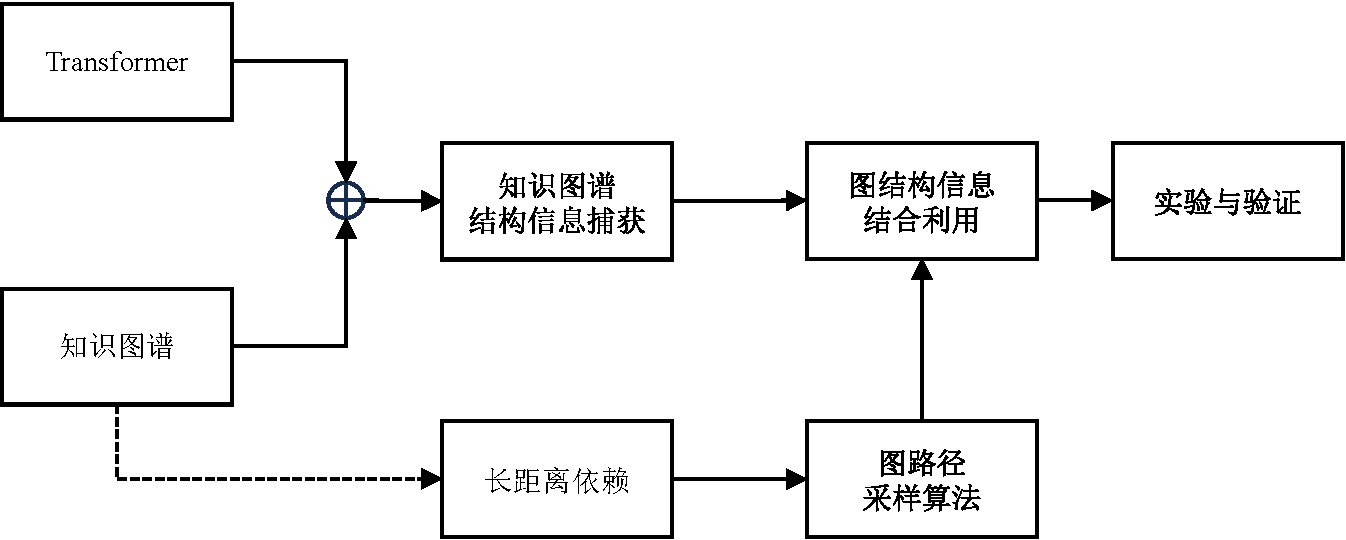
\includegraphics[width=0.9\textwidth]{pic/research_route_2.pdf}}
  \caption{研究路线示意图}
  \label{research_route}
\end{figure}

(1)基于Transformer的模型对于知识图谱结构的捕获研究

在Transformer中,任意一个位置都能直接感知到其他位置的输入信息,这导致模型无法直接捕捉到输入之间的相对位置关系,因此在处理序列数据时,采用的方式一般是为每个位置的输入添加对应的位置编码,标识输入与输入之间的前后位置关系。但在知识图谱中节点并不是顺序排列的,因此本文的主要研究内容之一就是设计一种合适方案让Transformer模型能够学习到知识图谱的拓扑结构,实现对知识图谱结构的感知。此外,在知识图谱中关系也是重要的结构信息,反映着实体和实体之间不同的交互方式,蕴含着丰富的语义信息,但标准的Transformer模型并没有直接的方式来编码和使用边的信息,因此Transformer如何对边信息进行表示也是重要的研究内容。

(2)图路径采样算法研究

针对基于图神经网络的方法对知识图谱中长距离信息学习不足的缺陷,本文计划通过对知识图谱中的图路径信息学习来挖掘实体与实体之间的长距离依赖,因此为了提升模型性能,对于当前的待遇测事实三元组,如何采样到高质量的图路径是首先需要解决的问题。因此本文计划研究设计合适的采样策略,实现高效的图路径采样,提高模型捕获长距离依赖的能力。

(3)不同图结构信息的结合方案研究

基于图神经网络的模型通过聚合消息的方式实现了对于中心实体局部邻域结构的感知,但无法捕捉实体之间长距离的依赖;基于图路径的方法能够挖掘到更远距离的依赖,但忽略了实体丰富的局部邻域。因此,本文的主要研究内容之一是设计合适的模型结构实现对于以上两类图结构信息的综合利用,实现对于图谱中长短距离信息的捕捉。

(4)实验与验证

在完成以上研究内容,实现完整的知识图谱补全模型之后,设计相应实验方案,通过平均排名、平均倒数排名等指标在主流公开数据集上与基线模型进行性能对比,验证本文提出的模型的有效性;并且通过设计合适的消融实验,验证模型关键设计的有效性。

\subsection{论文组织安排}
本文对基于Transformer的知识图谱补全方法进行研究,论文内容总共分为五个章节以及总结与展望部分,各个章节的内容安排组织如下:

第一章绪论首先介绍了论文的背景与意义,随后对知识图谱以及知识图谱算法的国内外研究进展进行了简单介绍,并进行了各类方法的对比与总结。随后明确了论文的研究目标与研究路线,概述了论文的主要研究内容。最后介绍了论文的组织安排。

第二章介绍了论文中方法所涉及到的相关理论基础。首先介绍了注意力机制与Transformer模型架构,其次对Transformer模型在图学习领域中的应用进行了概述,最后对不同类别的知识图谱嵌入方法进行了介绍,包括部分模型的核心思想以及数学公式。

第三章首先对Transformer模型在知识图谱嵌入领域的应用存在的困难进行了分析,随后介绍了提出的基于邻域感知Transformer的知识图谱补全模型,给出了符号定义以及模型的总体架构,并对其中的关键设计结构强化的自注意力机制进行了说明。

第四章首先指出了现有的基于图结构信息的方法的缺点,随后介绍了提出的结合图路径和局部邻域的Transformer知识图谱嵌入模型,说明了模型的总体架构以及各个模块的设计方案,包括基于有偏随机游走的图路径采样算法、图路径信息与局部邻域信息的结合方案以及掩蔽实体关系预测任务。

第五章为实验与验证部分,首先说明了实验采用的数据集、选取的进行对比的基线模型、实验环境以及采用的评估策略等基本情况,随后对实验结果进行了介绍和分析,包括本文提出的模型与基线模型的总体性能对比、关键模块消融实验的结果,超参数对于模型的性能影响等。

总结与展望部分对本文的研究内容进行了回顾与总结,并对未来可能的研究方向进行了展望。

\chapter{相关理论基础}
本章对论文中所涉及到的相关理论基础进行了介绍。首先介绍了注意力机制与Transformer模型架构,其次对Transformer模型在图表示学习领域中的应用进行了概述,最后对不同类型的知识图谱嵌入方法的核心思想和数学公式进行了说明,包括传统的知识图谱嵌入方法、基于图神经网络的知识图谱嵌入方法、基于图路径的知识图谱嵌入方法以及基于Transformer的知识图谱嵌入方法。

\section{注意力机制与Transformer网络}
深度学习中的注意力机制(Attention Mechanism)灵感来源于人类的视觉和认知系统。在推理过程中,注意力机制动态地为输入数据分配不同的权重,使模型能够自动地学习并选择性地关注输入中的重要信息,提高模型的性能和泛化能力。注意力机制最早被用于处理计算机视觉任务,后来在多个领域中得到了应用,例如自然语言处理和推荐系统等。

谷歌的研究团队于2017年提出的Transformer\upcite{Transformer}网络则是注意力机制方面里程碑式的工作。Transformer网络设计之初主要用于处理序列数据,在Transformer出现之前,序列数据的处理通常依赖于循环神经网络(RNN)及其变体,例如长短期记忆网络(LSTM)和门控递归单元(GRU)。RNN及其变体在处理序列数据时能够保持一定程度的历史信息,但存在一定的问题:由于对序列数据进行逐步处理,RNN在训练过程中容易出现梯度消失或者梯度爆炸的问题,特别是在处理长序列数据时。逐步处理也限制了模型的并行计算能力,导致训练效率低下。此外,尽管LSTM和GRU通过特殊的门控机制改善了长距离依赖问题,但当序列长度过高时,模型依然难以捕捉到距离较远的依赖关系。

Transformer\upcite{Transformer}网络通过使用自注意力(Self-Attention)机制解决了上述问题,在自注意力机制中,输入数据中的任意一个位置都能够直接感知到其它位置的信息,因此相比于传统的RNN结构,自注意力能够更加直接地捕捉到序列中长距离的依赖关系;自注意力机制允许模型在处理数据时并行计算各个位置的注意力分数,与RNN逐步计算的方式相比,可以显著提高模型的计算效率;自注意力机制通过学习输入序列中不同位置之间的动态相关性,能够根据特定的任务自适应地调整注意力分布。

Transformer\upcite{Transformer}网络中的自注意力机制的核心为缩放点积注意力机制,结构如图\ref{DotProductAttention}所示。
\begin{figure}[htbp]
  \vspace{-0.8cm}
  \centerline{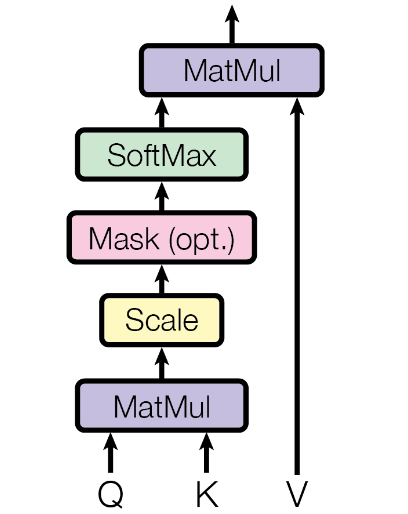
\includegraphics[width=0.250\textwidth]{pic/DotProductAttention.png}}
  \caption{缩放点积注意力机制}
  \label{DotProductAttention}
\end{figure}

具体来说,假设模型的输入为$X$,首先模型将会通过线性变化生成输入对应的查询向量$Q$,键向量$K$以及值向量$V$:
\begin{gather}
    Q=XW^Q, K=XW^K, V=XW^K
\end{gather}
其中$W^Q$、$W^K$、$W^K$是可学习的参数矩阵。

随后模型会将查询向量$Q$和键向量$K$进行点积并乘以缩放因子$\frac{1}{\sqrt{d_k}}$获得注意力分数,将其进行归一化处理转化为概率分布,用作权重对值向量$V$进行加权平均和,最终得到缩放点积注意力机制对应的输出,其中$d_k$为键向量的维度:
\begin{gather}
    \mbox{Attention}(Q,K,V) = \mbox{softmax}(\frac{QK^T}{\sqrt{d_k}})V
\end{gather}


进一步的,为了让模型能够同时关注来自不同维度的信息,并稳定自注意力的学习过程,Transformer采用了多头注意力机制,通过不同的参数矩阵将$Q$、$K$、$V$映射到不同的向量空间下并计算缩放点积注意力,将结果进行拼接获得最终的输出,如图\ref{MultiHeadAttention}所示。

具体来说,对于$h$个独立的注意力头,有:
\begin{equation}
  \begin{aligned}
    \mbox{MultiHead}(Q,K,V)&=\mbox{Concat}(head_1,...,head_h)W^O\\
    \mbox{where} \  head_i &=\mbox{Attention}(QW^Q_i,KW^K_i,VW^V_i)
  \end{aligned}
\end{equation}
其中$QW^Q_i$、$KW^K_i$、$VW^V_i$为将$Q$、$K$、$V$映射到第$i$个向量空间的参数矩阵,Concat为拼接操作。

\begin{figure}[htbp]
  \centerline{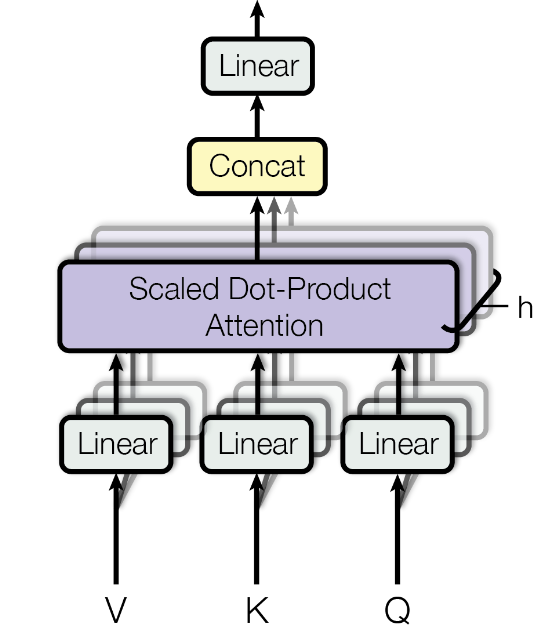
\includegraphics[width=0.3\textwidth]{pic/MultiHeadAttention.png}}
  \caption{多头注意力机制}
  \label{MultiHeadAttention}
\end{figure}
\section{基于Transformer的图表示学习方法}

图被广泛用于连接数据的网络结构表示,在社交系统、生态系统、生物网络、知识图谱等领域中都有广泛的应用。图表示学习方法将图的特征转化为低维嵌入空间中的向量。由于Transformer\upcite{Transformer}在计算机视觉和自然语言处理等领域展现出了出色的性能,近来,已经有大量的基于Transformer的模型被用于编码图结构数据。GraphTrans\upcite{GraphTrans}利用Transformer的自注意力机制学习图中的长距离的成对关系,并设计了一种读出机制以获得全局图嵌入。Grover\upcite{Grover}设计了节点级、边级和图级的自监督任务,能够从未标记的数据中学习图的结构和语义信息。Graphormer\upcite{Graphormer}对Transformer的注意力计算方式进行了改造,并从数学上证明了许多流行的图神经网络变体可以被视为Graphormer的特殊情况。

Graphormer\upcite{Graphormer}认为Transformer设计之初是为了建模序列数据,为了让其能够在图结构上实现最好效果,关键是要将图的结构信息恰当的融合到模型之中。Graphormer结合了几种有效的结构编码方法来利用这些信息。

Graphormer\upcite{Graphormer}认为Transformer模型中的注意力机制会基于节点的语义相似度计算注意力分布,因此提出了基于节点的出度和入度中心性编码来捕获知识图谱的节点重要性,其中$x_i$是节点表征,$z^-_{deg^-(v_i)}$和$z^+_{deg^+(v_i)}$是代表节点出度和入度的可学习表征:
\begin{equation}
  h_i^{(0)}=x_i+z^-_{deg^-(v_i)}+z^+_{deg^+(v_i)}
\end{equation}
Transformer模型在处理长序列文本时,会通过位置编码来学习文本之间的相对位置信息,但图不是序列数据,因此需要重新设计空间编码,加入到注意力运算中:
\begin{equation}
  A_{ij}=\frac{(h_iW_Q)(h_jW_K)^T}{\sqrt{d}}+b_{\varPhi (v_i,v_j)}
\end{equation}
这种编码方式的优势在于$b_{\varPhi (v_i,v_j)}$提供了一个对于图中的每个节点的全局的空间信息。

关系信息对于图中的节点表征至关重要,Graphormer\upcite{Graphormer}模型为了将关系信息加入到注意力中,引入了关系编码$c_{ij}$,表示的是节点$v_i$和$v_j$之间最短路径上所有关系表征的平均值,如下图公式所示:
\begin{equation}
  A_{ij}=\frac{(h_iW_Q)(h_jW_K)^T}{\sqrt{d}}+b_{\varPhi (v_i,v_j)}+c_{ij},\ \mbox{where} \ c_{ij} = \frac{1}{N}\sum_{n=1}^Nx_{e_n}(w_n^E)^T
\end{equation}
\section{知识图谱嵌入方法}

\subsection{传统的知识图谱嵌入方法}

传统知识图谱嵌入方法的研究对象是知识图谱中独立的三元组,集中于利用嵌入空间中的显式几何特性来捕捉实体之间的不同关系,基于翻译的方法、基于张量分解的方法和神经网络中的基于多层神经网络的、基于卷积神经网络的方法均属于此类。

基于翻译和基于张量分解的表示学习属于较早被提出的方法,它们模型结构简单,没有神经网络结构,计算速度快,可解释性较高。因此,在各个领域中的应用都十分广泛。

TransE\upcite{TransE}模型于2013年被提出,是基于翻译的知识图谱嵌入方法的起源。TransE的核心思想是将图谱中的关系视为嵌入空间内实体到实体的翻译,具体来说,TransE将实体和关系投影到相同的向量空间中,对于正确的事实三元组$(h,r,t)$,头实体嵌入$\boldsymbol{h}$和关系嵌入$\boldsymbol{r}$的相加结果应该尽可能得接近尾实体嵌入$\boldsymbol{t}$,即:
\begin{equation}
  \boldsymbol{h}+\boldsymbol{r}\approx \boldsymbol{t}
\end{equation}

而在TransE\upcite{TransE}的训练和评估过程中,对于训练集中的每一个正样本事实三元组$(h,r,t)$,TransE会通过随机替换头尾实体的方式,生成对应的负样本参与训练,这样的策略也成为了后续许多知识图谱嵌入方法的训练和评估策略。最终,对于扩充后的训练集中的每一个三元组$(h,r,t)$,TransE模型会计算$\boldsymbol{h}+\boldsymbol{r}$和$\boldsymbol{t}$之间的距离的L2范数作为衡量标准:
\begin{equation}
  d_r(h,t)=\left\lVert \boldsymbol{h}+\boldsymbol{r} - \boldsymbol{t}\right\rVert 
\end{equation}
对于正样本,TransE\upcite{TransE}期望得到的距离尽可能得小,负样本得到的距离尽可能的大,最终得到TransE模型的损失函数:
\begin{equation}
  \mathcal{L} =\sum_{(h,r,t)\in S}\sum_{(h^\prime,r,t^\prime)\in S^\prime_{(h,r,t)}}\left[\gamma +d_r(h,t)-d_r(h^\prime,t^\prime)\right] 
\end{equation}
其中$S$代表正样本集,$S^\prime_{(h,r,t)}$为生成的对应的负样本集。TransE方法最大的缺点是对复杂关系建模效果不佳,例如一对多、多对一以及多对多关系,容易把不同实体学习成相近的嵌入,随后的一系列基于翻译的方法针对这个缺点提出了很多的改进方式。

在基于张量分解的方法中,最为经典的是RESCAL\upcite{RESCAL}方法。给定一个知识图谱,RESCAL将其形式化为一个三阶张量${\mathcal{X} \in \mathbb{R}^{N \times N \times M}}$ ,其中$N$是实体的数量,$M$为关系种类的数量,张量的每一个切片$\mathcal{X}_k$对应于第$k$种关系的邻居矩阵,代表知识图谱中该种关系下实体之间的连接情况,如果实体$i$与实体$j$之间存在关系$k$,那么$\mathcal{X}_{ijk}$的值为1,否则为0。

RESCAL\upcite{RESCAL}假设每个实体$i$都可以通过一个向量$a_i \in \mathbb{R}^R$来表示,每类关系$k$由一个二维矩阵$R_k \in  \mathbb{R}^{R \times R}$表示,其中$R$为预定义的嵌入维度。RESCAL通过以下公式对张量$\mathcal{X}$进行分解:
\begin{equation}
  \mathcal{X}_k \approx A R_k A^T, \ \mbox{for} \ k=1,\ldots, m
\end{equation}
其中$A = [a_1,\ldots,a_N]$是实体嵌入矩阵。

RESCAL\upcite{RESCAL}模型的训练目标是最小化张量$\mathcal{X}$与通过学习到的实体和关系表示重建的张量之间的差异,因此模型的损失函数为:
\begin{equation}
  \min_{A,R_k} = f(A,R_k)+g(A,R_k)
\end{equation}
其中有:
\begin{equation}
  f(A,R_k)=\frac{1}{2}\left(\sum_k \left\lVert \mathcal{X}_k - AR_kA^T\right\rVert^2_F \right) 
\end{equation}
$g$为模型的正则项:
\begin{equation}
  g(A,R_k)=\frac{1}{2}\lambda \left(\left\lVert A\right\rVert^2_F+\sum_k\left\lVert R_k\right\rVert^2_F  \right) 
\end{equation}
其中$\left\lVert \cdot \right\rVert _F $为Frobenius范数,$\lambda$为正则化参数,用于防止过拟合。RESCAL\upcite{RESCAL}首次提出了基于张量分解的知识图谱嵌入方法,但也存在缺陷,用二维矩阵表示关系的方法使得RESCAL在处理大规模知识图谱时的计算成本和存储需求可能非常巨大,因此后续提出的一系列基于张量分解的方法在RESCAL的基础上进行了改进。

早期的基于神经网络的方法主要是采用多层神经网络来尝试直接拟合知识图谱。NTN\upcite{NTN}模型是一种用于知识图谱嵌入的神经网络架构,于2013年被提出。NTN通过引入张量运算和多层神经网络进行非线性特征变换来学习实体关系的语义信息,提高了模型的表达能力,克服了之前的知识图谱嵌入方法的限制。

NTN\upcite{NTN}模型采用低维向量代表实体,实体之间的关系则用一个三维张量进行表示。和RESCAL\upcite{RESCAL}模型类似,NTN引入了双线性张量操作。它通过在实体之间进行张量运算来捕捉实体之间的复杂交互关系,但是在NTN中还使用了基于多层神经网络的框架,相比于RESCAL,提供了更加丰富的线性特征表达能力。

在训练和评估过程中,NTN\upcite{NTN}通过以下公式来对事实三元组进行打分:
\begin{equation}
  f(h,r,t) = u_r^T \tanh\left(v_h^T M_r v_t + W_r^1v_h + W_r^2v_t + b_r\right) 
\end{equation}
其中,$v_h$和$v_t$分别为头实体和尾实体的嵌入向量,$u_r$为关系$r$的权重向量,$M_r$为关系$r$对应的三维张量,$W_r^1$和$W_r^2$为多层神经网络对应的线性变换矩阵,$b_r$为偏置项,$\tanh$为引入非线性的双曲正切激活函数。此外,NTN还采用了预训练的词向量来对实体和关系嵌入进行初始化,提升了模型的效果。

而随着卷积神经网络在计算机视觉领域大获成功,在知识图谱嵌入领域中也涌现出了以ConvE\upcite{ConvE}为代表的基于卷积神经网络的知识图谱嵌入方法。ConvE将设计和关系的嵌入表示重塑为二维矩阵,并用卷积神经网络来捕获实体和关系之间的复杂交互。具体来说,ConvE模型的具体计算步骤如下:

首先,对于给定的头实体$h$和关系$r$,ConvE\upcite{ConvE}将它们的嵌入重塑为二维形式,并拼接成一个二维矩阵:
\begin{equation}
  \left[\overline{\boldsymbol{h}};\overline{\boldsymbol{r}}\right] 
\end{equation}
其中$\left[;\right]$表示拼接操作,$\overline{\boldsymbol{h}}$和$\overline{\boldsymbol{t}}$表示头实体嵌入$\boldsymbol{h}$和关系嵌入$\boldsymbol{t}$重塑后的二维形式。

接下来ConvE\upcite{ConvE}对得到的二维矩阵进行卷积操作,应用ReLU激活函数$f$后得到的特征图为:
\begin{equation}
  f\left(\left[\overline{\boldsymbol{h}};\overline{\boldsymbol{r}}\right]\ast \omega\right)
\end{equation}
其中$\ast$表示卷积操作。随后ConvE将卷积层得到的特征图进行向量化,将得到的向量经过全连接层和ReLU激活函数后,形成最终的特征表示:
\begin{equation}
  f\left(\mbox{vec}\left(f\left(\left[\overline{\boldsymbol{h}};\overline{\boldsymbol{r}}\right]\ast \omega\right)\right)W\right)
\end{equation}
在预测阶段,模型将得到的特征表示与每个候选尾实体的嵌入进行点积得到对应的相似度得分:
\begin{equation}
  \psi_r(\boldsymbol{h},\boldsymbol{t})=f\left(\mbox{vec}\left(f\left(\left[\overline{\boldsymbol{h}};\overline{\boldsymbol{r}}\right]\ast \omega\right)\right)W\right)\boldsymbol{t}
\end{equation}
其中$\boldsymbol{t}$为尾实体嵌入。

最后,ConvE\upcite{ConvE}模型采用交叉熵损失函数对模型进行训练:
\begin{equation}
  \mathcal{L} (p,t)=-\frac{1}{N}\sum_i(t_i\cdot \log (p_i)+(1-t_i)\cdot\log(1-p_i))
\end{equation}
其中$p$为事实三元组正确的概率,有:
\begin{equation}
  p=\mbox{sigmoid}(\psi_r(\boldsymbol{h},\boldsymbol{t}))
\end{equation}

\subsection{基于图神经网络的知识图谱嵌入方法}
基于图神经网络的知识图谱嵌入方法是近些年知识图谱嵌入领域的一个重要发展方向,这类方法主要利用图神经网络的能力来学习图谱中实体和关系的嵌入表示。相比于传统的知识图谱嵌入方法,图神经网络天然适合处理图结构类型的数据,通过聚合一个实体周围的邻居节点信息来学习中心嵌入,这一过程能够捕捉到图谱中的局部拓扑信息,从而能够更好地表达实体之间的关系。此外,传统的嵌入模型往往只能考虑直接的实体关系,而图神经网络可以通过多层网络堆叠来捕捉实体之间的多跳路径信息,从而实现对更远距离实体关系的建模。

R-GCN\upcite{R-GCN}第一个在知识图谱嵌入领域应用图神经网络的方法。传统的图卷积网络主要设计用来处理无向图或者单一关系类型的图,但是这种方法无法直接应用于知识图谱,因为其忽略了图谱中边上的多种关系类型信息。而R-GCN则将图卷积神经网络扩展到了可以处理具有多种关系类型的图数据。R-GCN为图谱中的每种关系类型引入了一个单独的权重矩阵,每个关系类型在聚合邻居信息时能产生不同的影响,从而能够学习到每种关系特定的模式。R-GCN还在知识图谱中为每个实体添加了一个特殊类型的自环边,允许每个节点保留自身的信息,自环边在更新节点表示时作为单独的一种关系处理,也有自己的权重矩阵。

R-GCN\upcite{R-GCN}整体为编码器-解码器架构,使用改造后的图卷积神经网络作为编码器,使用DistMult\upcite{DistMult}方法作为链路预测任务的解码器,使用softmax函数来作为实体分类任务的解码器。

具体来说,R-GCN\upcite{R-GCN}的传播层用数学公式表示如下:
\begin{equation}
  h_i^{l+1}=\sigma \left(\sum_{r\in\mathcal{R}}\sum_{j\in\mathcal{N}_i^r}\frac{1}{c_{i,r}}W_r^lh_j^l+W_0^lh_i^l  \right) 
\end{equation}
其中$h_i^{l+1}$是第$i$个节点在经过第$l+1$层传播层更新后的表示,$\mathcal{N}_i^r$是节点$i$通过关系$r$相连接的邻居节点集合,$c_{i,r}$是归一化因子,一般设置为$c_{i,r}=\left\lvert\mathcal{N}_i^r\right\rvert$。

获得聚合后的实体表示后,R-GCN\upcite{R-GCN}使用DistMult\upcite{DistMult}方法对三元组进行打分:
\begin{equation}
  f(s,r,o)=e_s^TR_re_o
\end{equation}

训练用的损失函数为:
\begin{equation}
  \mathcal{L} =-\frac{1}{(1+\omega )\left\lvert\hat{\varepsilon } \right\rvert } \sum_{(s,r,o,y)\in \mathcal{T} }y\log l(f(s,r,o))+(1-y)\log(1-l(f(s,r,o)))
\end{equation}
其中$\omega$为R-GCN为每个正样本生成的负样本数量。
后续提出的基于图神经网络的方法在R-GCN的基础上进行了改进,基本沿用了R-GCN的编码器-解码器架构。SACN\upcite{SACN}将实体的邻域划分为带权值的子图进行聚合。TransGCN\upcite{TransGCN}提出了两种基于翻译的思想的编码器,分别用于实数域和复数域。

受到注意力机制在计算机视觉领域和自然语言处理领域的成功的启发,还有一部分基于图神经网络的方法尝试融合注意力机制。KBGAT\upcite{KBGAT}首次将图注意力网络用于知识图谱嵌入任务,RGHAT\upcite{RGHAT}使用实体和关系分层的方式对邻居的注意力进行了细分。

RGHAT\upcite{RGHAT}采用了一个创新的层次化注意力机制来充分利用实体的本地邻域信息,主要分为两层:关系级注意力根据不同关系对于中心实体重要性的不同为实体的每个邻接关系分配不同的权重;实体级注意力在关系级注意力的基础上进一步评估每个关系下邻居实体的重要性并分配对应的注意力分数。

对于中心实体$h$,邻接关系$r$的关系级注意力$\alpha_{h,r}$的计算方式如下:
\begin{gather}
  \mathbf{a}_{h,r} = \mathbf{W}_1\left[\mathbf{h}\Vert \mathbf{v}_r\right]\\
  \alpha_{h,r}=\mbox{softmax}_r(\mathbf{a}_{h,r})=\frac{\mbox{exp}(\sigma (\mathbf{p}\cdot \mathbf{a}_{h,r}))}{\sum_{r\prime \in \mathcal{N}_h }\mbox{exp}(\sigma(\mathbf{p}\cdot\mathbf{a}_{h,r^\prime}))}
\end{gather}
其中$\mathbf{h}$为实体$h$的嵌入,$\mathbf{W}_1$、$\mathbf{v}_r$和$\mathbf{p}$为可训练的参数,其中$\mathbf{v}_r$是关系特定的。

在关系级注意力的基础上,RGHAT进一步计算邻居节点$t$在关系$r$下对于中心实体$h$的实体级注意力$\beta_{r,t}$:
\begin{gather}
  \mathbf{b}_{h,r,t} = \mathbf{W}_2\left[\mathbf{a}_{h,r}\Vert \mathbf{t}\right]\\
  \beta_{r,t} = \mbox{softmax}_t(\mathbf{b}_{h,r,t}) = \frac{\mbox{exp}(\sigma(\mathbf{q}\cdot\mathbf{b}_{h,r,t}))}{\sum_{t\prime \in \mathcal{N}_{h,r}}\mbox{exp}(\sigma(\mathbf{q}\cdot \mathbf{b}_{h,r,t\prime}))} 
\end{gather}

之后将关系级注意力与实体级注意力相乘,RGHAT得到$(h,r,t)$在所有邻居三元组中的注意力得分$\mu_{h,r,t}$:
\begin{equation}
  \mu_{h,r,t} = \alpha_{h,r} \cdot \beta_{r,t}
\end{equation}

获得注意力得分之后,RGHAT\upcite{RGHAT}在每一层中对邻居信息进行聚合,结合中心实体自身的嵌入得到该层的输出:
\begin{gather}
  \hat{\mathbf{h}} = \sum_{r\in \mathcal{N}_h } \sum_{t\in\mathcal{N}_{h,r}}\mu_{h,r,t}\mathbf{b}_{h,r,t}\\
  \mathbf{h}^{'}  = \frac{1}{2}\left(\sigma(\mathbf{W}_3(\mathbf{h}+\hat{\mathbf{h}}))+\sigma(\mathbf{W}_4(\mathbf{h}\odot\hat{\mathbf{h}}))\right)
\end{gather}

RGHAT\upcite{RGHAT}还采用了多头注意力机制:
\begin{equation}
  \mathbf{h}^{'}=\mathop{\Vert}\limits_{k=1}^{K}\mathbf{h}^{'}_k
\end{equation}

通过采用层次化的注意力机制,RGHAT能够更精细地对实体的邻域进行建模,不仅聚焦于关系的重要性,还考虑了实体之间的语义贡献,提供了模型的可解释性。
\subsection{基于图路径的知识图谱嵌入方法}

和基于图神经网络的方法利用中心实体的局部邻域进行链路预测不同,基于图路径的方法则尝试学习图谱中的路径信息来捕获实体与实体之间的长距离依赖,PTransE\upcite{PTransE}、RSN\upcite{RSN}和Interstellar\upcite{Interstellar}模型均属于此类,其中PTransE是其中较早的方法。

PTransE\upcite{PTransE}建立在TransE\upcite{TransE}模型的基础上,并增加了考虑实体间多步关系路径的能力。PTransE的主要贡献在于它不仅仅考虑实体之间的直接关系,还考虑通过其他实体间接连接的路径,从而捕获更丰富的语义信息。

在PTransE中,路径由一系列关系构成,定义为:
\begin{equation}
  \mathbf{p} = \mathbf{r}_1\circ \cdots \circ \mathbf{r}_l
\end{equation}
其中$\circ$表示关系的串联。PTransE\upcite{PTransE}模型尝试学习路径$\mathbf{p}$的表示,可以通过多种方式实现,例如通过关系向量的相加、乘积或者利用循环神经网络来进行学习,目的是最小化以下距离函数:
\begin{equation}
  E(h,p,t)=\left\lVert \mathbf{p}-(\mathbf{t}-\mathbf{h})\right\rVert =\left\lVert \mathbf{p}-\mathbf{r}\right\rVert=E(p,r) 
\end{equation}

PTransE\upcite{PTransE}模型将直接关系和间接关系一同考虑,所以基于翻译的思想,以下距离函数也需要同时最小化:
\begin{equation}
  E(h,r,t)=\left\lVert \mathbf{h}+\mathbf{r}-\mathbf{t}\right\rVert 
\end{equation}
最终,PTransE\upcite{PTransE}模型的损失函数为:
\begin{equation}
  L(\mathbf{S})=\sum_{(h,r,t)\in \mathbf{S}}\left[L(h,r,t)+\frac{1}{Z}\sum_{p\in P(h,r)}R(p\vert h,t)L(p,r)\right] 
\end{equation}
其中$R(p\vert h,t)$为路径的置信度,$L(h,r,t)$和$L(p,r)$为基于间隔的损失函数:
\begin{equation}
  L(h,r,t)=\sum_{(h^{'},r^{'},t^{'})\in \mathbf{S}^-}\left[\gamma +E(h,r,t)-E(h^{'},r^{'},t^{'})\right]_+ 
\end{equation}
\begin{equation}
  L(p,r)=\sum_{(h,r^{'},t)\in \mathbf{S}^-}\left[\gamma +E(p,r)-E(p,r^{'})\right]_+
\end{equation}

通过结合直接关系和通过多步路径发现的间接关系,PTransE\upcite{PTransE}能够捕捉实体之间更为复杂的交互模式,从而提高知识图谱补全任务的性能。但是,PTransE没有考虑到路径中的实体信息,因此后面提出的基于路径的知识图谱补全方法对PTransE进行了改进。
\subsection{基于Transformer的知识图谱嵌入方法}

基于Transformer\upcite{Transformer}的知识图谱嵌入方法的核心思路是利用Transformer强大的表达能力来挖掘图谱中的语义和结构信息,以学习知识图谱的嵌入表示。Transformer模型的自注意力机制能够有效地捕捉实体之间的复杂关系和交互。还可以通过在Transformer中集成额外信息进一步加强实体和关系的表示。代表方法有HittER\upcite{HittER}和Relphormer\upcite{Relphormer}。

Relphormer\upcite{Relphormer}是一种为知识图谱嵌入任务而设计的基于Transformer的神经网络架构。为了解决知识图谱中实体与关系节点的异构性,Relphormer把实体和关系均视为相同的节点,有$ V=\mathcal{E} \cup \mathcal{R}$为节点集合,其中$\mathcal{E}$为实体集合,$\mathcal{R}$为关系集合,并用邻接矩阵$\mathbf{A} \in\left\{0,1\right\}^{\left\lvert V\right\rvert\times \left\lvert V\right\rvert} $来表示节点之间的连接关系,事实三元组表示为:$\mathcal{T} =(v_s,v_p,v_o)$,中心节点的局部邻域为:
\begin{equation}
  \mathcal{T}_G = \mathcal{T}_c \cup \mathcal{T}_{context}, \ \mbox{where} \ \mathcal{T}_{context} =\left\{\mathcal{T}_i\in\mathcal{N} \right\} 
\end{equation}
由于Transformer是序列数据模型,Relphormer利用Triple2Seq算法对中心节点的局部邻域进行随机采样,抽取一部分邻接三元组并转化对应的为序列数据。

由于知识图谱是图结构,为了防止局部邻域转化为序列数据后损失知识图谱的结构信息,Relphormer\upcite{Relphormer}提出了一种结构强化的自注意力机制,当计算注意力分数时,额外添加一个偏差项:
\begin{equation}
  a_{ij}=\frac{(\mathbf{h}_i\mathbf{W}_Q)(\mathbf{h}_j\mathbf{W}_K)}{\sqrt{d}}+\phi (i,j)
\end{equation}
\begin{equation}
  \phi (i,j)=f_{structure}(\tilde{\mathbf{A}^1},\tilde{\mathbf{A}^2},\cdots,\tilde{\mathbf{A}^m} )
\end{equation}
其中$\tilde{\mathbf{A}}$是归一化后的邻接矩阵,$\tilde{\mathbf{A}^m}$是$\tilde{\mathbf{A}}$的$m$次方,指在$m$步内节点的连通性。

对于一些较为密集的知识图谱,每步训练中对局部邻域的随机采样过程随机性较大,可能会导致训练过程中的不一致性。为了避免这个问题,Relphormer利用上下文对比策略来克服不稳定性,使用不同训练步骤中相同三元组的采样的局部邻域的内容来强制模型进行类似的预测,最小化以下损失函数:
\begin{equation}
  \mathcal{L}_{contextual} = -\log\frac{\mbox{exp}(\mbox{sim}(\boldsymbol{c}_t,\boldsymbol{c}_{t-1})/\tau )}{\mbox{exp}(\mbox{sim}(\boldsymbol{c}_t,\boldsymbol{c}_{t-1})/\tau )+\sum_j\mbox{exp}(\mbox{sim}(\boldsymbol{c}_t,\boldsymbol{c}_{j})/\tau )}
\end{equation}
其中$\tau$为温度系数,$\boldsymbol{c}_t$为第$t$步采样到的样本的表示,$\mbox{sim}(\boldsymbol{c}_t,\boldsymbol{c}_{t-1})$为$\boldsymbol{c}_t$与$\boldsymbol{c}_{t-1}$之间的余弦相似度:$\frac{\boldsymbol{c}_t^T\boldsymbol{c}_{t-1}}{\left\lVert \boldsymbol{c}_{t}\right\rVert \cdot \left\lVert \boldsymbol{c}_{t-1}\right\rVert }$。

受掩码语言模型例如BERT\upcite{BERT}的启发,和之前的知识图谱嵌入方法不同,Relphormer\upcite{Relphormer}采用了一种新的训练策略:随机掩盖输入序列中的特定节点,然后对其进行预测。具体来说,在训练过程中,随机遮掩中心三元组头实体或者尾实体,并利用剩余的节点序列$\mathcal{T}_M$和上下文邻接矩阵$\mathbf{A}_G$的情况下,预测缺失的部分$Y$:
\begin{equation}
  \begin{aligned}
    &\mathcal{T}_M = MASK(\mathcal{T}_G)\\
    &Relphormer(\mathcal{T}_M,\mathbf{A}_G)\rightarrow Y
  \end{aligned}
\end{equation}

最终,Relphormer\upcite{Relphormer}模型的损失函数为:
\begin{equation}
  \mathcal{L}_{all} = \mathcal{L}_{MKM}+\lambda \mathcal{L}_{contextual}
\end{equation}
其中$\mathcal{L}_{MKM}$和$\mathcal{L}_{contextual}$分别为掩盖预测任务和上下文对比任务的损失函数。


\section{本章小结}

本章对论文中所涉及到的相关理论基础和关键技术进行了介绍,方便后续章节的说明。首先对注意力机制与Transformer模型的原理进行介绍,然后介绍了Transformer网络在图表示学习中的应用,最后介绍了知识图谱嵌入方法,包括不利用图结构的传统的知识图谱嵌入方法,以及基于图神经网络的知识图谱嵌入方法、基于图路径的知识图谱嵌入方法和基于Transformer的知识图谱嵌入方法。

\chapter{基于邻域感知的Transformer模型}


本章主要对NATLP模型的总体设计和模块的具体实现进行了介绍。主要包括对现存基于图神经网络方法存在问题的分析、模型的总体框架设计、关系特定的邻居实体信息构造设计以及融合图结构信息的自注意力机制的改进。
% Transformer网络虽然在自然语言处理(NLP)领域取得了巨大成功,但在直接应用到图表示学习(Graph Representation Learning)领域时会遇到一系列挑战和困难。图表示学习涉及到处理图数据,图数据具有非欧几里得结构,这与NLP中处理的序列数据(一维结构)有本质区别。下面列举了一些Transformer在图表示学习中面临的主要困难:

% 1. **非序列结构**:图是一种无序的数据结构,节点之间的关系是通过边来定义的,并且没有固定的顺序。相比之下,Transformer网络原本是为处理序列数据设计的,它使用位置编码来保留序列中元素的顺序信息。在图中,节点没有自然的顺序,因此Transformer网络无法直接使用位置编码来捕捉节点间的结构关系。

% 2. **邻居多样性**:在图中,每个节点可能有不同数量的邻居。这种动态的、不规则的邻接关系与Transformer网络中假设的固定大小的输入上下文不相符。因此,直接应用自注意力机制来学习图节点表示时难以处理不同节点的可变邻居数量。

% 3. **长距离依赖**:尽管Transformer网络擅长捕捉长距离依赖,但在图中,这种依赖通常是通过节点之间的路径来定义的,而不是序列中的线性位置。因此,Transformer需要被修改或扩展,以便能够理解和利用图中的路径和结构模式。

% 4. **缩放问题**:对于大型图,使用Transformer进行全图的自注意力学习是计算资源密集型的,因为复杂度是图中节点数量的平方。这使得直接在大规模图上应用Transformer变得不切实际。

% 5. **边的信息和类型**:在图中,边可能包含重要的信息,并且边的类型(如社交网络中的不同关系类型)也可能对图表示至关重要。然而,标准的Transformer模型并没有直接的方式来编码和使用边的信息。

% 为了克服这些困难,研究人员已经提出了许多不同的方法和模型的变种,如图注意力网络(Graph Attention Networks, GATs)和图Transformer网络(Graph Transformer Networks),这些模型专门设计或修改以适应图数据的特性。这些变种通常包括对自注意力机制的修改,以更好地处理图的结构性质,以及引入适合于图结构的新型位置编码或相对位置编码。此外,为了处理大型图,研究人员还在探索如何有效地对图进行采样,以及如何利用稀疏性和分层结构来降低计算复杂度。

% Transformer在知识图谱嵌入任务中具有以下优点:

% 1. 处理长距离依赖关系:知识图谱中的实体和关系之间存在着复杂的长距离依赖关系。传统的基于图的模型(如Graph Convolutional Networks)往往只考虑局部邻居信息,难以捕捉到远距离的语义依赖。而Transformer通过自注意力机制可以处理全局上的依赖关系,能够更好地捕捉实体和关系之间的长距离语义关联。

% 2. 并行计算能力:与循环神经网络不同,Transformer网络可以进行并行计算,加快了训练和推理的速度。在大规模的知识图谱中,由于实体和关系的数量庞大,传统的基于图的模型可能面临计算效率低下的问题,而Transformer网络能够更高效地处理大规模的知识图谱数据。

% 3. 对复杂属性建模:知识图谱中的实体通常具有丰富的属性信息,如文本描述、分类标签等。传统的基于图的模型往往无法有效地捕捉和利用这些属性信息,而Transformer网络可以将这些属性信息作为输入,并通过多头注意力机制对不同属性进行建模,从而更好地捕捉实体的语义特征。

% 4. 高度可扩展性:Transformer网络可以通过增加层数和调整参数来提高模型的表示能力。在知识图谱嵌入任务中,复杂的语义关系和多层次的结构需要一个具有较强建模能力的模型来学习。Transformer网络的多层结构可以提供更强的表示能力,可以通过增加层数来适应不同任务的需求。

% 综上所述,Transformer在知识图谱嵌入任务中具有处理长距离依赖关系、并行计算能力、对复杂属性建模和高度可扩展性等优点,为知识图谱的表示学习提供了一种强大而灵活的模型选择。

%注意力中添加度数:1-1/度数乘积

\section{现有问题描述和分析}

图卷积神经网络GCN于2017年被提出,对原先图神经网络中基于谱空间的的图卷积算子进行了优化,降低了模型的复杂度,由此引发了图神经网络的研究热潮。图神经网络迅速成为了图结构数据处理的重要方式,在社交网络\upcite{social}、推荐系统、知识图谱等多个领域都有着重要应用。近几年,图神经网络的应用是知识图谱嵌入领域非常重要的进展。图卷积神经网络能够直接处理图结构数据并捕捉知识图谱中的拓扑结构,通过聚合邻居节点的信息,图神经网络可以有效地学习知识图谱中节点(实体)和边(关系的嵌入表示)。相较于之前的方法,基于图神经网络的知识图谱嵌入方法获得了很大的性能提升。

然而,受限于本身的网络结构,在进行知识图谱嵌入时,基于图神经网络的方法依然存在不足,导致其性能受限。首先,图卷积神经网络采用聚合邻居节点的方法来更新中心实体的表示,在这个过程中,模型只考虑了邻居节点和中心实体之间的连通性,却忽略了不同邻居节点之间的可能也存在直接连接,各个邻居节点传递的信息之间是互不感知、互相独立的,这样的聚合方式没有将邻居节点信息之间的相互依赖纳入考虑;其次,图神经网络采用的消息传递模式整体模型结构比较简单,使模型的表达能力受到了限制,在挖掘图谱中实体和实体、实体与关系之间的复杂交互上存在困难。

而在以上两个方面,Transformer网络存在巨大的优势。首先,通过构造查询向量、键向量和值向量来进行注意力的计算以及采用多头注意力机制,相比于图神经网络,Transformer能够更加高效地挖掘输入之间各个维度的复杂交互;同时,通过调整模型的层数、头的数量或是隐层的维度大小,Transformer可以很容易地适应处理不同规模和复杂度的知识图谱的需求。

其次,Transformer网络的自注意力机制能够有效地捕捉序列中任意两个元素之间的全局依赖关系。在知识图谱嵌入的场景之中,这意味着模型在挖掘局部邻域的结构信息时,除了邻居节点和中心节点之间的依赖之外,还能够同时学习到邻居节点之间的长距离依赖,捕获邻居节点传递的信息之间的相互影响。此外,Transformer架构还支持模型的预训练和迁移学习,可以首先在一个大规模的综合性知识图谱上进行预训练,然后迁移到特定领域的知识图谱上,通过这样的方式,可以减少模型对标注数据的依赖,提高模型在特定任务上的表现。

但是,虽然Transformer网络在自然语言处理(NLP)领域已经取得了巨大成功,但将Transformer网络直接应用到知识图谱嵌入领域时依旧会遇到一系列挑战和困难。图具有非欧几里得结构,是一种无序的数据结构,这与NLP中处理的序列数据(一维结构)有本质区别。Transformer网络原本是为处理序列数据设计的,它使用位置编码来保留序列中元素的顺序信息。但是,在知识图谱中,节点之间的关系是通过边来定义的,并且没有固定的顺序,因此Transformer网络无法直接使用位置编码来捕捉节点间的结构关系。部分方法例如MAGNN\upcite{MAGNN}选择通过随机游走的方式来将图数据转化为序列数据来处理,但这样的方式会导致图结构信息的失真。

此外,在知识图谱中,边,即关系,反映着实体和实体之间不同的交互方式,蕴含着丰富的语义信息。两个实体之间连接的关系不同,传递的信息可能是千差万别的,因此如何采用合适的方式来对利用关系信息,体现关系对于消息传递的影响十分重要。但标准的Transformer模型并没有直接的方式来编码和使用边的信息。部分利用Transformer来进行知识图谱表示学习的模型例如Relphormer\upcite{Relphormer}将知识图谱中的实体和关系视为地位相同的节点,采用同样的方式进行处理,这样的方式虽然解决了边的表示问题,但没有考虑到知识图谱中实体和关系的差异性,没有考虑到关系对于实体消息传递的独特作用。

为了解决上述问题,本章提出了一种基于邻域感知的Transformer模型用于链路预测任务(Neighborhood Aware Transformer for Link Prediction, NATLP)。首先,在模型输入信息构造阶段,为了充分建模不同关系对于实体传递消息的影响,模型基于关系生成特定的网络参数,实现关系特定的邻居信息构造。其次,为了让Transformer能够更好地处理图结构数据,模型对Transformer的自注意力机制进行了改造,提出了一种融合图结构的自注意力机制,使得Transformer能够学习到输入消息之间的互相依赖。

\section{NATLP模型设计}

\subsection{符号定义}

为了方便说明论文提出的NATLP模型的实现细节,本节首先对模型中的关键概念和相关的数学符号进行了定义,具体内容参见表\ref{definition}。

\setlength{\tabcolsep}{20pt}

\begin{longtable}[htbp]{cc}
  % 首页表头
  \caption{NATLP模型中的符号定义}
  \label{definition}\\
  \toprule
  符号  & 说明\\
  \midrule
  \endfirsthead
  % 续页表头
  \caption{NATLP模型中的符号定义}\\
  \toprule
  符号  & 说明 \\
  \midrule
  \endhead
  % 首页表尾
  \hline
  % \multicolumn{2}{r}{\small 续下页}
  \endfoot
  % 续页表尾
  \bottomrule
  \endlastfoot
  $\mathcal{G}$   &   知识图谱      \\
  $\mathcal{E}, \mathcal{R}, \mathcal{T}$   &   实体集合、关系集合、边集合      \\
  $\mathcal{G}^\prime$  &  拓展后的知识图谱      \\
  $\mathcal{R}^{\prime}$   &   拓展后的关系集合      \\
  $\mathcal{T}^{-1}$   &   逆关系边集合      \\
  $\mathcal{T}^{\prime}$   &   拓展后的边集合      \\
  $(s,r,?)$  &   待遇测的三元组      \\
  $s$   &   头实体即中心实体      \\
  $o$   &   尾实体即目标实体      \\
  $e$   &   实体      \\
  $r$   &   关系      \\
  $r^{-1}$   &   关系$r$的逆关系      \\
  $\boldsymbol{s},\boldsymbol{o}$ & 头实体嵌入和尾实体嵌入\\
  $\boldsymbol{e},\boldsymbol{r}$ & 实体嵌入和关系嵌入\\


\end{longtable}

知识图谱是表示为$(s,r,o)$的“头实体-关系-尾实体”事实三元组的集合,所有的这些事实三元组连接起来构成了一个异构图,即为知识图谱,表示为$\mathcal{G} = (\mathcal{E}, \mathcal{R}, \mathcal{T})$,其中$\mathcal{E}$集合,$\mathcal{R}$为关系集合,$\mathcal{R}$为实体和关系构成的边集合。由于知识图谱中的关系具有方向性,为了确保信息能够在两个相连的实体之间进行双向的流通,本文在知识图谱中为每个事实三元组$(s,r,o)$创建了对应的逆三元组$(o,r^{-1},s)$,其中$r^{-1}$是关系$r$对应的逆关系。因此,关系集合、边集合以及知识图谱被拓展为:
\begin{gather}
    \mathcal{R}^{\prime}=\mathcal{R}\cup\{ r^{-1} | r\in \mathcal{R}\}\\
    \mathcal{T}^{-1}= \{ (o,r^{-1},s)| (s,r,o)\in \mathcal{T}\}\\
    \mathcal{T}^{\prime} = \mathcal{T}\cup\mathcal{T}^{-1}\\
    \mathcal{G}^\prime = (\mathcal{E}, \mathcal{R}^\prime, \mathcal{T}^\prime)
\end{gather}

知识图谱补全任务,即链路预测任务,是在给定待遇测三元组中的头实体$s$以及关系$r$的情况下预测缺失的尾实体$o$,表示为$(s, r, ?)$,或者是在给定尾实体$o$以及逆关系$r^{-1}$的情况下预测缺失的头实体$s$,表示为$(?, r^{-1} , o) $。为了方便说明,论文随后统一采用$(s, r, ?)$的形式进行表述。


\subsection{模型总体结构}

本节主要对提出的用于链路预测的基于邻域感知的Transformer模型NATLP的总体结构进行介绍。NATLP整体为编码器-解码器架构,编码器部分主要由关系特定的邻居信息构造模块和邻域感知Transformer模块组成,解码器部分则采用了基于卷积神经网络的知识图谱嵌入方法进行了实现。模型整体架构如图所示。

编码器的主要作用是将模型输入的实体和关系转化为对应的嵌入,并学习其中蕴含的语义信息和结构信息并编码成向量形式,是模型的核心部分。在NATLP中,模型的输入主要包括待预测的三元组及其局部邻域,编码器首先会根据中心实体和邻居之间相连的关系种类,为每一个邻居实体构造关系特定的邻居消息;随后的邻域感知Transformer模块综合学习构造的邻居信息、中心实体本身的信息以及局部邻域的结构信息,并完成编码。

解码器的主要任务则是根据编码器得到的知识表示,对下游任务的各项性能指标进行评测。根据下游任务的不同,模型可以采用不同的解码器进行解码。NATLP采用了基于卷积神经网络的知识图谱嵌入方法ConvE作为解码器,来对事实三元组的正确概率进行评估,完成知识图谱补全。

\subsection{关系特定的邻居信息构造}

链路预测任务的目标是利用知识图谱中已有的事实去预测未知事实在知识图谱中的存在概率,为了能够充分利用邻域信息来帮助预测三元组中缺失的尾实体,模型需要获得局部邻域中邻居实体向中心实体传递的信息。

而知识图谱中的关系反映着实体和实体之间不同的交互方式,对实体之间传递的信息有着很大的影响。因此,NATLP首先会基于邻居实体和连接的关系,完成邻居实体的消息构造。

因此在完成数据的预处理之后,模型的下一步任务是将已有的事实转化为模型能够接受的形式作为输入。

类似的设计在基于图神经网络的知识图谱嵌入方法中也



\chapter{NALTP模型实验与验证}

为了证明本课题提出的NATLP算法以及相关的关键设计能够有效提高知识图谱补全任务的性能,本文在标准数据集上进行了实验验证。本章首先对NALTP的实验方案设计进行了介绍,包括实验采用的数据集、实验环境、评估策略;用来对比的基线算法以及模型在两个数据集上的超参数设置;随后对模型的实验结果进行了分析和讨论,包括整体性能分析、关键设计分析。

\section{实验方案设计}

\subsection{实验数据集}
为了对NATLP模型进行评估,本文在两个标准基准数据集FB15k-237\upcite{FB15k-237}和WN18RR\upcite{ConvE}上进行了实验。FB15k-237是开源知识图谱Freebase\upcite{freebase}的子集,存储了有关电影、演员、奖项等等现实世界的常识信息的。WN18RR则是开源知识图谱WordNet\upcite{wordnet}的子集,包含了英文单词中的语义信息,例如同义、反义、单词概念的上下层等多种单词语义关系。为了避免测试集出现逆关系泄露的问题,两个数据集中所有的逆关系都已经被去除。两个数据集的统计数据如表\ref{dataset_statistics}所示,其中训练集用于模型参数训练,验证集用于模型超参数调优,测试集用于模型性能评估。值得注意的是,这两个数据集中的关系数量存在差异,FB15k-237包含了237种Freebase中的不同关系,而WN18RR的关系种类数量为11,总的来说,相比于FB15k-237,WN18RR数据集更加的稀疏。

\begin{table}[htbp]
  \renewcommand\arraystretch{1.5}
  \caption{数据集统计信息}
  \centering
  \begin{tabular}{*{3}{c}}
    \toprule
    数据集 & FB15k-237 & WN18RR\\
    \midrule
    \#实体数量  & 10541 & 40943 \\
    \#关系数量 & 237 & 11\\
    \#训练集数量 & 272115 &86835\\
    \#验证集数量 &17535 &3034\\
    \#测试集数量 &20466 &3134\\
    \#实体平均度数 &42.7 &4.5\\
    \bottomrule
  \end{tabular}
  \label{dataset_statistics}
\end{table}

\subsection{实验评估策略}

知识图谱的链路预测任务被定义为实体排序预测任务。测试集中的每个三元组将在两种不同的场景中进行链路预测评估:给定头实体和关系下的尾实体预测$(s,r,?)$,以及给定尾实体和关系下的头实体预测$(?,r,o)$。在实践中,头实体预测以$(o,r^-1,?)$的形式执行。预测时,待预测的头实体或者尾实体将被每个候选实体替换,并计算每个候选三元组的得分,随后所有的候选三元组将按照分数降序进行排序,以获得基本事实三元组的准确排名,并根据排名来对评估指标进行计算。

在知识图谱补全任务中,平均排名(Mean Rank,MR)、倒数平均排名(Mean Reciprocal Rank,MRR)和前N名百分比(Hits@n)三种评估指标将用来评估模型的性能。假设测试集中待预测三元组的数量为$K$,$rank_i$为第$i$个三元组的正确实体在所有候选实体中的排序位置,则平均排序MR的计算方式为:
\begin{equation}
    MR = \frac{\sum_i rank_i}{K}
\end{equation}
MR代表了所有正确实体的平均排序位置,MR越小,说明正确实体的得分越高,排名越靠前,模型的性能更好。但是MR存在的最大问题则是它对于不同排序位置的预测效果投入的关注是一样的,例如,假设有两个三元组,其中一个三元组的正确实体的排名从105上升到了100,另一个三元组的正确实体的排名从5上升到了1,他们对于MR指标的贡献是一致的,但是一般来说,在实验中我们认为从5到1的提升是更有意义的,平均排名指标MR则忽略了这一点。

平均倒数排名MRR对于这个问题进行了改进,MRR计算的时候正确实体排名的倒数的平均值,而不是排名的平均值,具体计算公式为:
\begin{equation}
    MRR = \frac{1}{K} \sum_i \frac{1}{rank_i}
\end{equation}
通过这样的计算方式,排名越靠前的项会获得更大的权重占比,对于整体性能指标的贡献越大。和MR不同,MRR越高,代表模型的性能越好。

前N名百分比Hits@n指的则是所有测试三元组中正确实体的排序处于前n名的比例,计算方式为:
\begin{equation}
    Hits@n = \frac{\sum_i \left[1 \ if \ rank_i \leq n \ or \ 0\right] }{K}
\end{equation}
指标越高,代表模型的性能越好。在知识图谱补全任务中,常用的前N名百分比指标包括Hits@1,Hits@3和Hits@10。

此外,注意到对于一个待预测的三元组$(s,r,?)$,正确实体$o$的选项可能不止一个,例如(姚明,出生于,上海)和(姚明,出生于,中国)都是正确的事实。在计算评价指标时,其余的正确实体可能会导致当前测试三元组中的正确实体排名下降,对模型评估造成影响,因此本文和大多数基线模型类似,计算排序时除了基本事实三元组之外的所有正确三元组都被排除在排名之外。

\subsection{实验环境}

本文采用的实验环境中的服务器硬件和软件配置如表\ref{environment}所示。硬件配置方面,实验所采用的服务器的处理器规格为Intel(R) Core(TM) i9-10920X CPU @ 3.50GHz,内存大小为128G,使用的显卡型号为GeForce RTX 4090,对应的显存大小为24G;软件配置方面,使用的操作系统为Ubuntu 5.4.0-74,采用的编程语言为Python,版本为3.10.9,使用的深度学习框架及其对应的版本为Pytorch 1.13.1。

\begin{table}[htbp]
    \renewcommand\arraystretch{1.5}
    \caption{采用的实验环境}
    \centering
    \begin{tabular}{*{2}{c}}
      \toprule
      配置项目 & 版本/内容\\
      \midrule
      处理器  & Intel(R) Core(TM) i9-10920X CPU @ 3.50GHz \\
      内存 & 128G\\
      显卡 & GeForce RTX 4090\\
      显存 & 24G\\
      操作系统 & Ubuntu 5.4.0-74\\
      编程语言 & Python 3.10.9\\
      深度学习框架 & Pytorch 1.13.1\\
      \bottomrule
    \end{tabular}
    \label{environment}
\end{table}


\subsection{对比算法}

为了验证本文提出的NATLP方法在知识图谱补全任务上的有效性,实验部分本文选取了一些最具代表性的以及最先进的知识图谱补全方法作为基线模型与NATLP模型进行了对比实验,主要包含以下几类方法:

(1)基于翻译的知识图谱嵌入模型,包括TransE\upcite{TransE},RotatE\upcite{RotatE}。

(2)基于张量分解的知识图谱嵌入模型,包括DistMult\upcite{DistMult},ComplEx\upcite{ComplEx}。
 
(3)基于卷积神经网络的模型,包括ConvE\upcite{ConvE},ConvR\upcite{ConvR}。

(4)基于图神经网络的知识图谱嵌入模型,包括R-GCN\upcite{R-GCN},CompGCN\upcite{CompGCN},KBGAT\upcite{KBGAT},HKGN\upcite{HKGN},SE-GNN\upcite{SE-GNN}以及MRGAT\upcite{MRGAT}。

\subsection{超参数设置}

NATLP模型在实验中采用的超参数是通过网格搜索在验证集上进行评估后得出的,主要涉及到的超参数有实体和关系嵌入的维度、关系特定的邻居实体信息构造中使用的卷积核的大小、卷积核的数量、不同神经网络层的Dropout概率、训练批次的大小、训练中的总迭代次数、训练中的最大学习率以及标签的平滑比例等。

实验中采用了Adamax\upcite{Adamax}优化器结合动态学习率调整策略进行模型的训练。在总迭代次数的前10\%内,模型的学习率将从0线性提升到最高,并在剩余迭代次数内线性下降到0。为了防止模型出现过度自信的现象,训练过程中以0.1的比率进行了标签平滑。NATLP模型在两个数据集上的具体的超参数设置见表\ref{NALTP_hyperparameter}所示。

\begin{table}[htbp]
  \renewcommand\arraystretch{1.5}
  \caption{NATLP模型超参数设置}
  \centering
  \begin{tabular}{*{3}{c}}
    \toprule
    超参数 & FB15k-237 & WN18RR\\
    \midrule
    实体和关系嵌入大小  & 320 & 320 \\
    卷积核大小 & 3$\times$3 & 3$\times$3\\
    卷积核数量 & 32 & 32\\
    Transformer网络层数& 4 & 4\\
    嵌入层Dropout概率 & 0.2 & 0.2\\
    Transformer中的Dropout概率 & 0.6 & 0.6\\
    训练批次大小 & 512 & 512\\
    总迭代次数& 300 & 500 \\
    最大学习率 & 0.001 & 0.02\\
    标签平滑比例 & 0.1 & 0.1\\
    \bottomrule
  \end{tabular}
  \label{NALTP_hyperparameter}
\end{table}

\section{实验结果与分析}

\subsection{整体实验结果分析}

不同模型在WN18RR数据集和FB15k-237数据集上的链路预测实验结果如表\ref{NATLP_result_tab}所示。文献\cite{49}在充分大的超参数搜索空间下采用统一的训练框架进行了大量的实验,探究了不同训练策略、模型架构和超参数搜索方法对于知识图谱嵌入模型性能的影响,发现如果选择合适的训练方法,许多浅层的知识图谱嵌入模型能够获得比原始文献中优秀得多的性能。因此TransE,RotatE,DistMult,ComplEx和ConvE模型在两个数据集上的实验结果直接选取文献\cite{49}中经过大量调参后的最优结果。另外,文献\cite{50}指出KBGAT中存在评估策略不当以及测试集数据泄露的问题,因此KBGAT的实验结果选取自文献\cite{50}中经过修正后的结果。

\begin{table}[htbp]
  \begin{center}
      \caption{NATLP实验结果}
      \renewcommand\arraystretch{1.5}
      \setlength{\tabcolsep}{5pt}
      \begin{tabular}{*{11}{c}}
          \toprule
          \multirow[vpos]{2}{*}[-0.8ex]{模型} & \multicolumn{5}{c}{WN18RR} & \multicolumn{5}{c}{FB15k-237}\\
          \cmidrule(lr){2-6}\cmidrule(lr){7-11}
          &MRR & MR & Hits@1 &Hits@3 & Hits@10&MRR & MR & Hits@1 &Hits@3 & Hits@10\\
          \midrule
          TransE&0.228&-&0.053&0.368&0.520&0.313&-&0.221&0.347&0.497\\
          RotatE&0.478&-&0.439&0.494&0.553&0.333&	-&0.240&0.368&0.522\\
          \cmidrule{1-11}
          DistMult&0.452&-&0.413&0.466	&0.530	&0.343	&-	&0.250	&0.378	&0.531\\
          ComplEx&0.475&-&0.438	&0.490	&0.547	&0.348	&-	&0.253	&0.384	&0.536\\
          \cmidrule{1-11}
          ConvE&0.442&-&0.411&0.451	&0.504&	0.339	&-&	0.248&	0.369	&0.521\\
          ConvR&0.475&-&0.443&	0.489&	0.537&	0.350&	-&	0.261&	0.385&	0.528\\
          \cmidrule{1-11}
          R-GCN & -&-&-&-&-&0.248&-&0.153&0.258&0.414\\
          CompGCN&0.479&3533&0.443	&0.494	&   0.546&	0.355	&197	&0.264	&0.390&	0.535\\
          KBGAT&0.412&\textbf{1921}&-&	-&	0.554	&0.157	&270	&-&	-&	0.331\\
          SE-GNN&0.484&3211&0.446&	\underline{0.509}&	\underline{0.572}	&\underline{0.365}& \textbf{157}	&\underline{0.271}	&\underline{0.399}	&\underline{0.549}\\
          MRGAT&0.481&-&0.443&0.501&0.568&0.358	&-&0.266&0.386&0.542\\
          HKGN&\underline{0.487}&\underline{2468}&\underline{0.448}&0.505&0.561&\underline{0.365}&194&\underline{0.271}&0.397&0.544\\
          \cmidrule{1-11}
          \textbf{NATLP}&\textbf{0.505}&2687&\textbf{0.465}&\textbf{0.519}&\textbf{0.576}&\textbf{0.374}&\underline{181}&\textbf{0.281}&\textbf{0.411}&\textbf{0.560}\\
          % TKGE-PN&\textbf{0.510}&2540&\textbf{0.467}	&\textbf{0.522}	&\underline{0.590}	&\textbf{0.379}	&160	&\underline{0.288}	&\textbf{0.414}	&\textbf{0.562}\\
          \bottomrule
      \end{tabular}
      \label{NATLP_result_tab}
  \end{center}
\end{table}

表中加粗项为每项指标的最高值,下划线项为每项指标的次高值。从表\ref{NATLP_result_tab}中可以观察到,在两个基准数据集的绝大多数指标上,NATLP都取得了最优的效果,相对于次优结果,在FB15k-237数据集上,NATLP在MRR、Hits@1、Hits@3和Hits@10四个指标上分别取得了3.6\%,3.7\%, 1.9\%, 0.6\%的性能提升;在WN18RR数据集上,NATLP在MRR、Hits@1、Hits@3和Hits@10四个指标上分别取得了2.4\%,3.6\%, 3.0\%和2.0\%的性能提升,这表明相比于基线模型,本文提出的NALTP方法在链路预测任务上有着更好的表现,证明了NATLP模型的有效性。同样使用了注意力机制,相比于HKGN以及MRGAT等基于图神经网络的方法,NATLP有着可观的性能提升,证明了Transformer网络强大的表达能力以及在知识图谱嵌入领域的应用潜力。

\subsection{模型关键设计分析}

为了验证NATLP模型中关键设计:关系特定的邻居实体信息构造以及邻域感知Transformer模块的有效性,本文进行了多方面的对比实验来验证关键设计的效果。

首先,为了验证关系特定的邻居实体信息构造中参数生成网络以及全局关系嵌入对于链路预测任务的作用,本文在两个数据集上分别以三种设置进行了消融实验,分别是(1)原始NATLP模型,未对模型进行任何改动;(2)消融了参数生成网络的NATLP模型,同一实体在不同关系下进行信息构造中共享完全相同的网络参数;(3)消融了全局关系嵌入的NATLP模型,参数生成网络仅依赖于关系嵌入进行参数生成。实验结果如表\ref{NATLP_ablation1}所示。

\begin{table}[htbp]
  \begin{center}
      \caption{关系特定的邻居实体信息构造消融实验}
      \setlength{\tabcolsep}{8pt}
      \renewcommand\arraystretch{1.5}
      % \renewcommand{\arraystretch}{1}
      \begin{tabular}{*{7}{c}}
          \toprule
          数据集 & 模型设置 & MRR&MR&Hits@1&Hits@3&	Hits@10\\
          \midrule
          \multirow{3}{*}{WN18RR}&NATLP&0.505&2504&0.466&0.519&0.578\\
          &消融参数生成网络&0.496&2399&0.456&0.512&0.575\\
          &消融全局关系嵌入&0.503&2519&0.461&0.518&0.578\\
          \cmidrule{1-7}
          \multirow{3}{*}{FB15k-237}&NATLP&0.376&161&0.284&0.411&0.561\\
          &消融参数生成网络&0.367&145&0.274&0.404&0.555\\
          &消融全局关系嵌入&0.373&175&0.279&0.411&0.558\\
          \bottomrule
      \end{tabular}
      \label{NATLP_ablation1}
  \end{center}
\end{table}

从表\ref{NATLP_ablation1}中实验结果可以观察到,在对参数生成网络进行消融后,模型的在两个数据集上的链路预测性能都有了明显的下降,这证明了相比于采用统一的网络参数进行消息构造,关系特定的网络参数能够更好地捕捉实体中关系相关的特定特征,挖掘相关的语义信息,提高任务性能;注意到消融了参数生成网络之后,相比于WN18RR数据集上的表现,NATLP模型在FB15k-237数据集上的性能下降更为严重,本文认为这样的差异主要是由于两个数据集上的关系种类差异所导致的,FB15k-237数据集中的关系种类为237种,远远超过WN18RR数据集上的11种,因此采用统一的网络参数时模型在FB15k-237数据集上损失的信息更多。此外,去除全局关系嵌入后模型在两个数据集上的性能也有所下降,证明了捕捉关系之间共同特征的有效性。

此外,为了验证邻域感知Transformer模块中基于实体节点间最短距离的偏置项以及基于节点度数的偏置项的有效性,本文在两个数据集上以四种设置进行了NATLP模型的消融实验,分别是(1)原始NATLP模型,未对模型进行任何改动;(2)消融了基于实体节点间最短距离的偏置项的NATLP模型;(3)消融了基于节点度数的偏置项的NATLP模型;(4)同时对两个偏置项进行了消融的NATLP模型。具体实验结果如表\ref{NATLP_ablation2}所示。

\begin{table}[htbp]
  \begin{center}
      \caption{邻域感知Transformer模块消融实验}
      \setlength{\tabcolsep}{8pt}
      \renewcommand\arraystretch{1.5}
      % \renewcommand{\arraystretch}{1}
      \begin{tabular}{*{7}{c}}
          \toprule
          数据集 & 模型设置 & MRR&MR&Hits@1&Hits@3&	Hits@10\\
          \midrule
          \multirow{4}{*}{WN18RR}&NATLP&0.505&2504&0.466&0.519&0.578\\
          &消融节点最短距离的偏置项&0.500&2603&0.457&0.515&0.573\\
          &消融节点度数偏置项&0.501&2570&0.459&0.517&0.578\\
          &消融两个偏置项&0.497&2856&0.454&0.515&0.570\\
          \cmidrule{1-7}
          \multirow{4}{*}{FB15k-237}&NATLP&0.376&161&0.284&0.411&0.561\\
          &消融节点最短距离的偏置项&0.373&180&0.280&0.409&0.557\\
          &消融节点度数偏置项&0.372&184&0.281&0.409&0.554\\
          &消融两个偏置项&0.369&179&0.277&0.409&0.550\\
          \bottomrule
      \end{tabular}
      \label{NATLP_ablation2}
  \end{center}
\end{table}

通过表中结果可以发现,无论是消融了节点间最短距离的偏置项还是节点度数的偏置项,模型在两个数据集上的性能都会出现下降,证明了两种结构信息对于链路预测任务的重要性。


\section{本章小结}

本章对于基于领域感知的Transformer模型NALTP的实验部分进行了介绍,首先对本文中实验的基本方案设计进行了说明,包括实验采用的数据集,模型的评估策略以及实验的硬件和软件环境,并介绍了用来对比NATLP的基线模型。随后论文对NALTP模型的整体实验结果进行了介绍,相对于次优结果,在FB15k-237数据集上,NATLP在MRR、Hits@1、Hits@3和Hits@10四个指标上分别取得了3.6\%,3.7\%, 1.9\%, 0.6\%的性能提升;在WN18RR数据集上,NATLP在MRR、Hits@1、Hits@3和Hits@10四个指标上分别取得了2.4\%,3.6\%, 3.0\%和2.0\%的性能提升,证明了NATLP模型的性能表现优于绝大部分现有的模型;最后通过消融实验对NATLP模型的中的关键设计:关系特定的邻居实体信息构造以及邻域感知Transformer模块进行了深入的探究和分析,证明了通过显式捕捉关系对于实体消息传递的影响,以及在自注意力机制中编码知识图谱图结构能够有效地提高模型的链路预测任务性能。

\chapter{结合图路径和局部邻域的Transformer模型}

% 本章主要对结合图路径和局部邻域的Transformer模型TKGE-PN的总体设计和模块的具体实现进行了介绍。主要包括对基于图神经网络的方法以及NATLP模型存在问题的分析、模型的总体框架设计、基于有偏随机游走的图路径采样算法的设计、Path-Transformer路径编码模块以及Neighbor-Transformer局部邻域编码模块的具体设计。

本文提出的NATLP模型通过关系特定的邻居实体信息构造和邻域感知Transformer模块提高了模型的表达能力,获得了优异的知识图谱补全性能,但是由于主要利用局部邻域信息进行预测,和基于图神经网络的方法类似,依然存在对图谱中长距离依赖学习不足的问题。针对以上问题,本文基于前文提出的NATLP模型,尝试利用知识图谱的图路径结构来学习图谱中的长距离依赖,进一步提出了提出了一种基于Transformer的结合图路径和局部邻域的知识图谱嵌入方法(A Transformer-based Knowledge Graph Embedding Model Combining Graph Paths and Local Neighborhood,TKGE-PN)。

\section{现有问题分析}
NATLP模型对传统的Transformer模型的自注意力机制的计算方式进行改进,捕获了中心实体局部邻域内的结构信息,将Transformer模型应用到了知识图谱补全中,解决了先前基于图神经网络的方法模型表达能力差、对邻居实体之间相互依赖学习不足的问题。

但是,NATLP模型依然存在缺陷,由于依然基于中心实体的局部邻域进行推理,NATLP并没有解决基于图神经网络的知识图谱嵌入方法对于于长距离依赖学习不足的缺点。在知识图谱中,长距离的含义是实体间通过边连接需要经过多个中间节点。长距离依赖反映出实体之间较为间接的联系,这种联系在理解实体间复杂关系的层面上是非常重要的。例如,某一个历史人物与某一个现代组织之间可能存在长距离依赖,尽管他们之间直接的联系很少,但通过一系列历史事件和影响,可以构建出两者之间的联系,因此捕捉长距离依赖有益于推理和查询知识图谱的高阶模式。

基于图神经网络的方法主要是通过利用中心实体的局部邻域中蕴含的信息来完成知识图谱的补全。每层图神经网络只能学习到中心实体的一跳邻居的信息,这导致模型能够很好的捕捉知识图谱中的短距离依赖,而对于实体和实体之间的长距离依赖的学习不够充分。虽然其可以通过堆叠多层图神经网络让中心实体感知到距离更远的其他实体,但这样的方式只在层数较低(例如一到两层)时有效,之后随着层数的进一步增加,模型的性能反而会出现快速的下降,这主要是由过平滑问题(over-smoothing)导致的,即因为感受野的重叠而导致不同节点的表示过于相似无法进行区分。文献\cite{over-smoothing}对这种现象进行了系统和定量的研究,通过引入定量指标,发现导致过平滑的关键因素是节点接收到的有效信息与噪声比例过低,结果如图\ref{information-noise}所示,该图来自于文献\cite{over-smoothing}原文。在每层神经网络中,节点都会聚合其所有邻居节点的信息并传递给下一层,这导致模型引入了大量的噪声信息。因此基于图神经网络的方法一般只能捕捉单个实体附近1-2跳内的局部信息,而缺乏利用长距离乃至全局信息的能力。
\begin{figure}[htb]
  \centerline{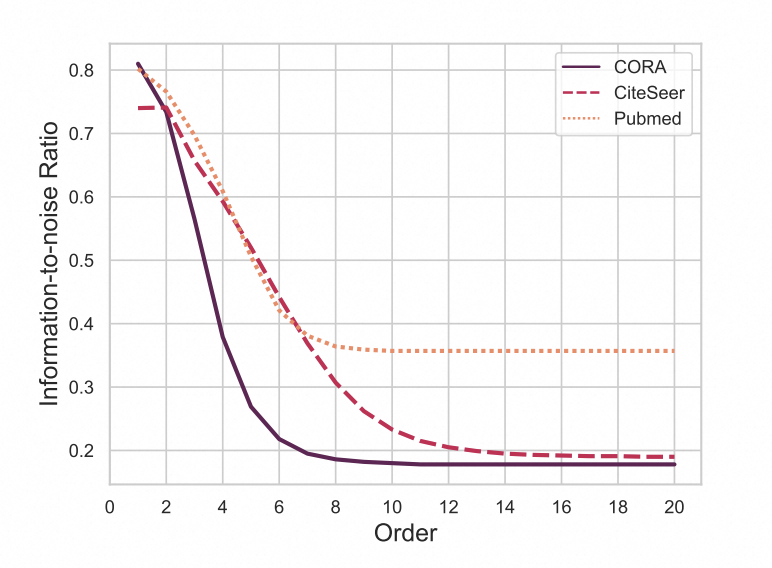
\includegraphics[width=0.7\textwidth]{pic/information-noise.png}}
  \caption{网络层数对信噪比的影响}
  \label{information-noise}
\end{figure}

为了解决以上问题,本文提出了一种基于Transformer的结合图路径和局部邻域的知识图谱嵌入方法(A Transformer-based Knowledge Graph Embedding Model Combining Graph Paths and Local Neighborhood,TKGE-PN)。基于图神经网络的方法的成功证明了实体的局部邻域蕴含了丰富的信息,但知识图谱的结构信息除了图神经网络使用的局部邻域之外还有多种表达形式,例如图路径以及子图。在知识图谱中,图路径被定义为图谱中的实体-关系链,由不同三元组收尾相连组成,例如(Yao Ming, Born In, Shanghai, City Of, China)。相对于局部邻域,图路径能够帮助模型更好地捕获实体和实体之间长距离的依赖,如图\ref{long-term-dependency}所示。结合图路径和邻域信息,模型能够更好地学习长短距离依赖的同时避免过度平滑问题的出现。同样的,和NATLP类似,和GNN浅层的神经网络结构相比,Transformer的自注意力机制能够给模型带来更强大的表达能力。本文提出的TKGE-PN以中心实体作为起点,采用有偏随机游走算法对图路径进行采样,并通过基于Transformer的图路径编码模块Path-Transformer和邻域信息编码模块Neighbor-Transformer对图谱中的长距离和短距离结构信息进行编码。此外针对相比于近距离的信息,长距离信息学习更为困难的问题,本文为图路径编码模块设计了一个掩蔽实体关系预测任务,以确保模型能够充分学习图路径之间的长距离依赖。

\begin{figure}[htb]
    \centerline{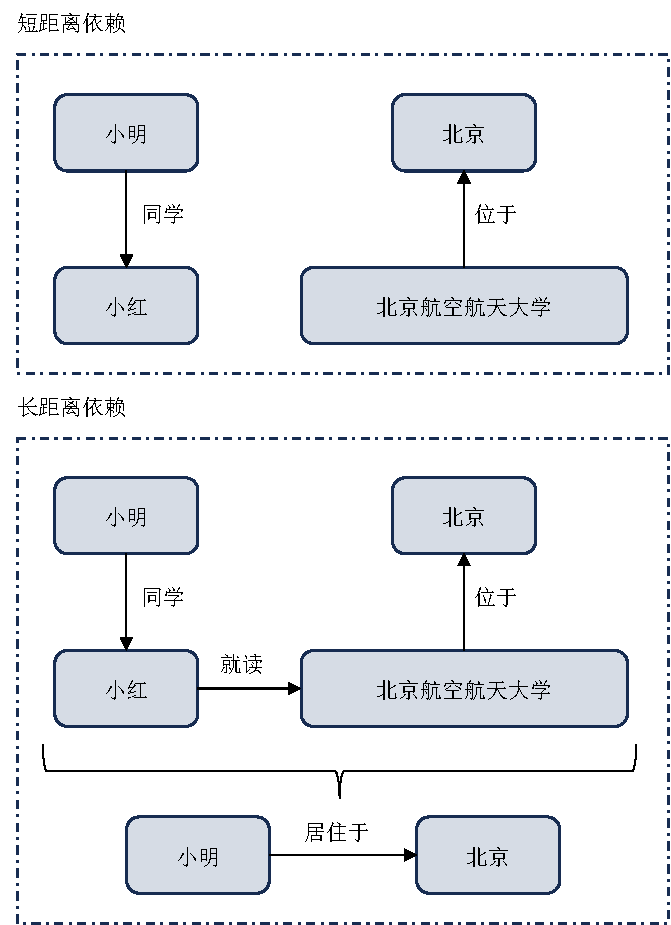
\includegraphics[width=0.5\textwidth]{pic/long-term-dependency.pdf}}
    \caption{知识图谱中的短距离信息和长距离信息}
    \label{long-term-dependency}
  \end{figure}

\section{TKGE-PN模型设计}

\subsection{符号定义}
为了方便说明论文提出的TKGE-PN模型的实现细节,本节对TKGE-PN模型中的关键概念和相关的数学符号进行了定义,具体内容参见表\ref{definition_TKGE-PN}。

\setlength{\tabcolsep}{20pt}

\renewcommand\arraystretch{1.2}
\begin{longtable}[htbp]{cc}
  % 首页表头
  \caption{TKGE-PN模型中的符号定义}
  \label{definition_TKGE-PN}\\
  \toprule
  符号  & 说明\\
  \midrule
  \endfirsthead
  % 续页表头
  \caption{TKGE-PN模型中的符号定义}\\
  \toprule
  符号  & 说明 \\
  \midrule
  \endhead
  % 首页表尾
  \hline
  % \multicolumn{2}{r}{\small 续下页}
  \endfoot
  % 续页表尾
  \bottomrule
  \endlastfoot
  
  $\mathcal{G}$   &   知识图谱      \\
  $\mathcal{E}, \mathcal{R}, \mathcal{T}$   &   实体集合、关系集合、边集合      \\
  $\mathcal{G}^\prime$  &  拓展后的知识图谱      \\
  $\mathcal{R}^{\prime}$   &   拓展后的关系集合      \\
  $\mathcal{T}^{-1}$   &   逆关系边集合      \\
  $\mathcal{T}^{\prime}$   &   拓展后的边集合      \\
  $(s,r,?)$  &   待遇测的三元组      \\
  $s$   &   头实体即中心实体      \\
  $o$   &   尾实体即目标实体      \\
  $e$   &   实体      \\
  $r$   &   关系      \\
  $r^{-1}$   &   关系$r$的逆关系      \\
  $\boldsymbol{s},\boldsymbol{o}$ & 头实体嵌入和尾实体嵌入\\
  $\boldsymbol{e},\boldsymbol{r}$ & 实体嵌入和关系嵌入\\
  $T$ & 图路径的长度\\
  $P$ & 知识图谱中的图路径\\
  $\mathcal{N}_s$ & 实体 $s$的一阶邻居节点集合\\
  $\mu_{depth}(e_{i+1})$ & 候选实体$e_{i+1}$的深度偏差\\
  $\mu_{degree}(e_{i+1})$ & 候选实体$e_{i+1}$的度数偏差\\
  $\alpha$ & 控制深度偏差的权重\\
  $\beta$ & 控制度数偏差的权重\\
  $p_{sample}$ & 采样过程中实体被选中的概率\\
  $e_m,r_m$ & 掩蔽实体关系预测任务中被掩蔽的实体或关系\\
  $\mathbf{M}_{input}^{P},\mathbf{M}_{output}^{P}$ & Path-Transformer模块的输入和输出\\
  $\boldsymbol{e}_{mask}$ & 掩蔽占位嵌入\\
  $\boldsymbol{e}_{query}$ & 查询向量\\
  $d$ & 嵌入维度\\
  $\phi_{chk}$ & 棋盘式特征重组\\
  $\circledast$ & 循环卷积操作\\
  $f(\cdot )$ & ReLU激活函数\\
  $vec(\cdot)$ & 二维张量转化为一维向量\\
  $\omega_r$ & 特定于关系$r$的卷积层参数\\
  $\mathbf{W}_r$ &特定于关系$r$的全连接层参数\\
  $\boldsymbol{e}_{cls}$ & Path-Transformer特殊嵌入Class Token\\
  $\boldsymbol{e}_{gcls}$ & Neighbor-Transformer特殊嵌入Global Class Token\\
  $\mathbf{TE}$ & 类型嵌入\\
  $\mathbf{PE}$ & 位置嵌入\\
  $a_{ij}$ & 第i个输入和第j个输入之间的注意力得分\\
  $dis(e_i,e_j)$ & 实体$e_i$与实体$e_j$之间最短路径的距离\\
  $deg(e)$ & 实体$e$的节点度数\\
  $\boldsymbol{o}_t$ & 模型预测的候选实体的嵌入\\
  $\sigma $ & sigmoid激活函数\\
  $p$ & 三元组正确概率\\
  $L_{MERP}$ & 掩蔽实体关系预测任务的损失\\
  $L_{LP}$ & 链路预测任务损失\\
  $L$ & 模型损失\\
  $t_i$ & 第i个三元组的标签\\

\end{longtable}

和NATLP中的处理方式类似,为了确保实体之间信息的双向流动,TKGE-PN会对原始的知识图谱进行拓展,为知识图谱中的每个事实三元组$(s,r,o)$添加对应的逆关系$r^{-1}$和逆三元组$(o,r^{-1},s)$:

\begin{gather}
    \mathcal{R}^{\prime}=\mathcal{R}\cup\{ r^{-1} | r\in \mathcal{R}\}\\
    \mathcal{T}^{-1}= \{ (o,r^{-1},s)| (s,r,o)\in \mathcal{T}\}\\
    \mathcal{T}^{\prime} = \mathcal{T}\cup\mathcal{T}^{-1}\\
    \mathcal{G}^\prime = (\mathcal{E}, \mathcal{R}^\prime, \mathcal{T}^\prime)
\end{gather}

\subsection{模型总体结构}

本节主要对提出的基于Transformer的结合图路径和局部邻域的知识图谱嵌入方法TKGE-PN的总体结构进行介绍。模型架构如图\ref{TKGE-PN_architecture}所示。

和NATLP不同,TKGE-PN并没有采用编码器-解码器架构,而是利用Transformer自身的强大表达能力直接对目标实体的嵌入进行预测,这样的方式的优点是模型可以充分发挥自注意力机制的强大表达能力,其性能不会受限于用作解码器的基于图神经网络的知识图谱嵌入方法的限制。

TKGE-PN模型主要由三个核心部分组成。首先第一部分是基于有偏随机游走的图路径采样算法,主要职责是以中心实体为起点在图谱中采样多条图路径;随后第二部分Path-Transformer路径编码模块负责学习采样到的图路径中蕴含的长距离的语义信息并将其转换为向量表示;最后Neighbor-Transformer局部邻域编码模块接收来自Path-Transformer的输入,整合待遇测事实三元组中的信息以及多条图路径所构成上下文邻域信息,并以此预测三元组得分。

\begin{figure}[htbp]
  \centerline{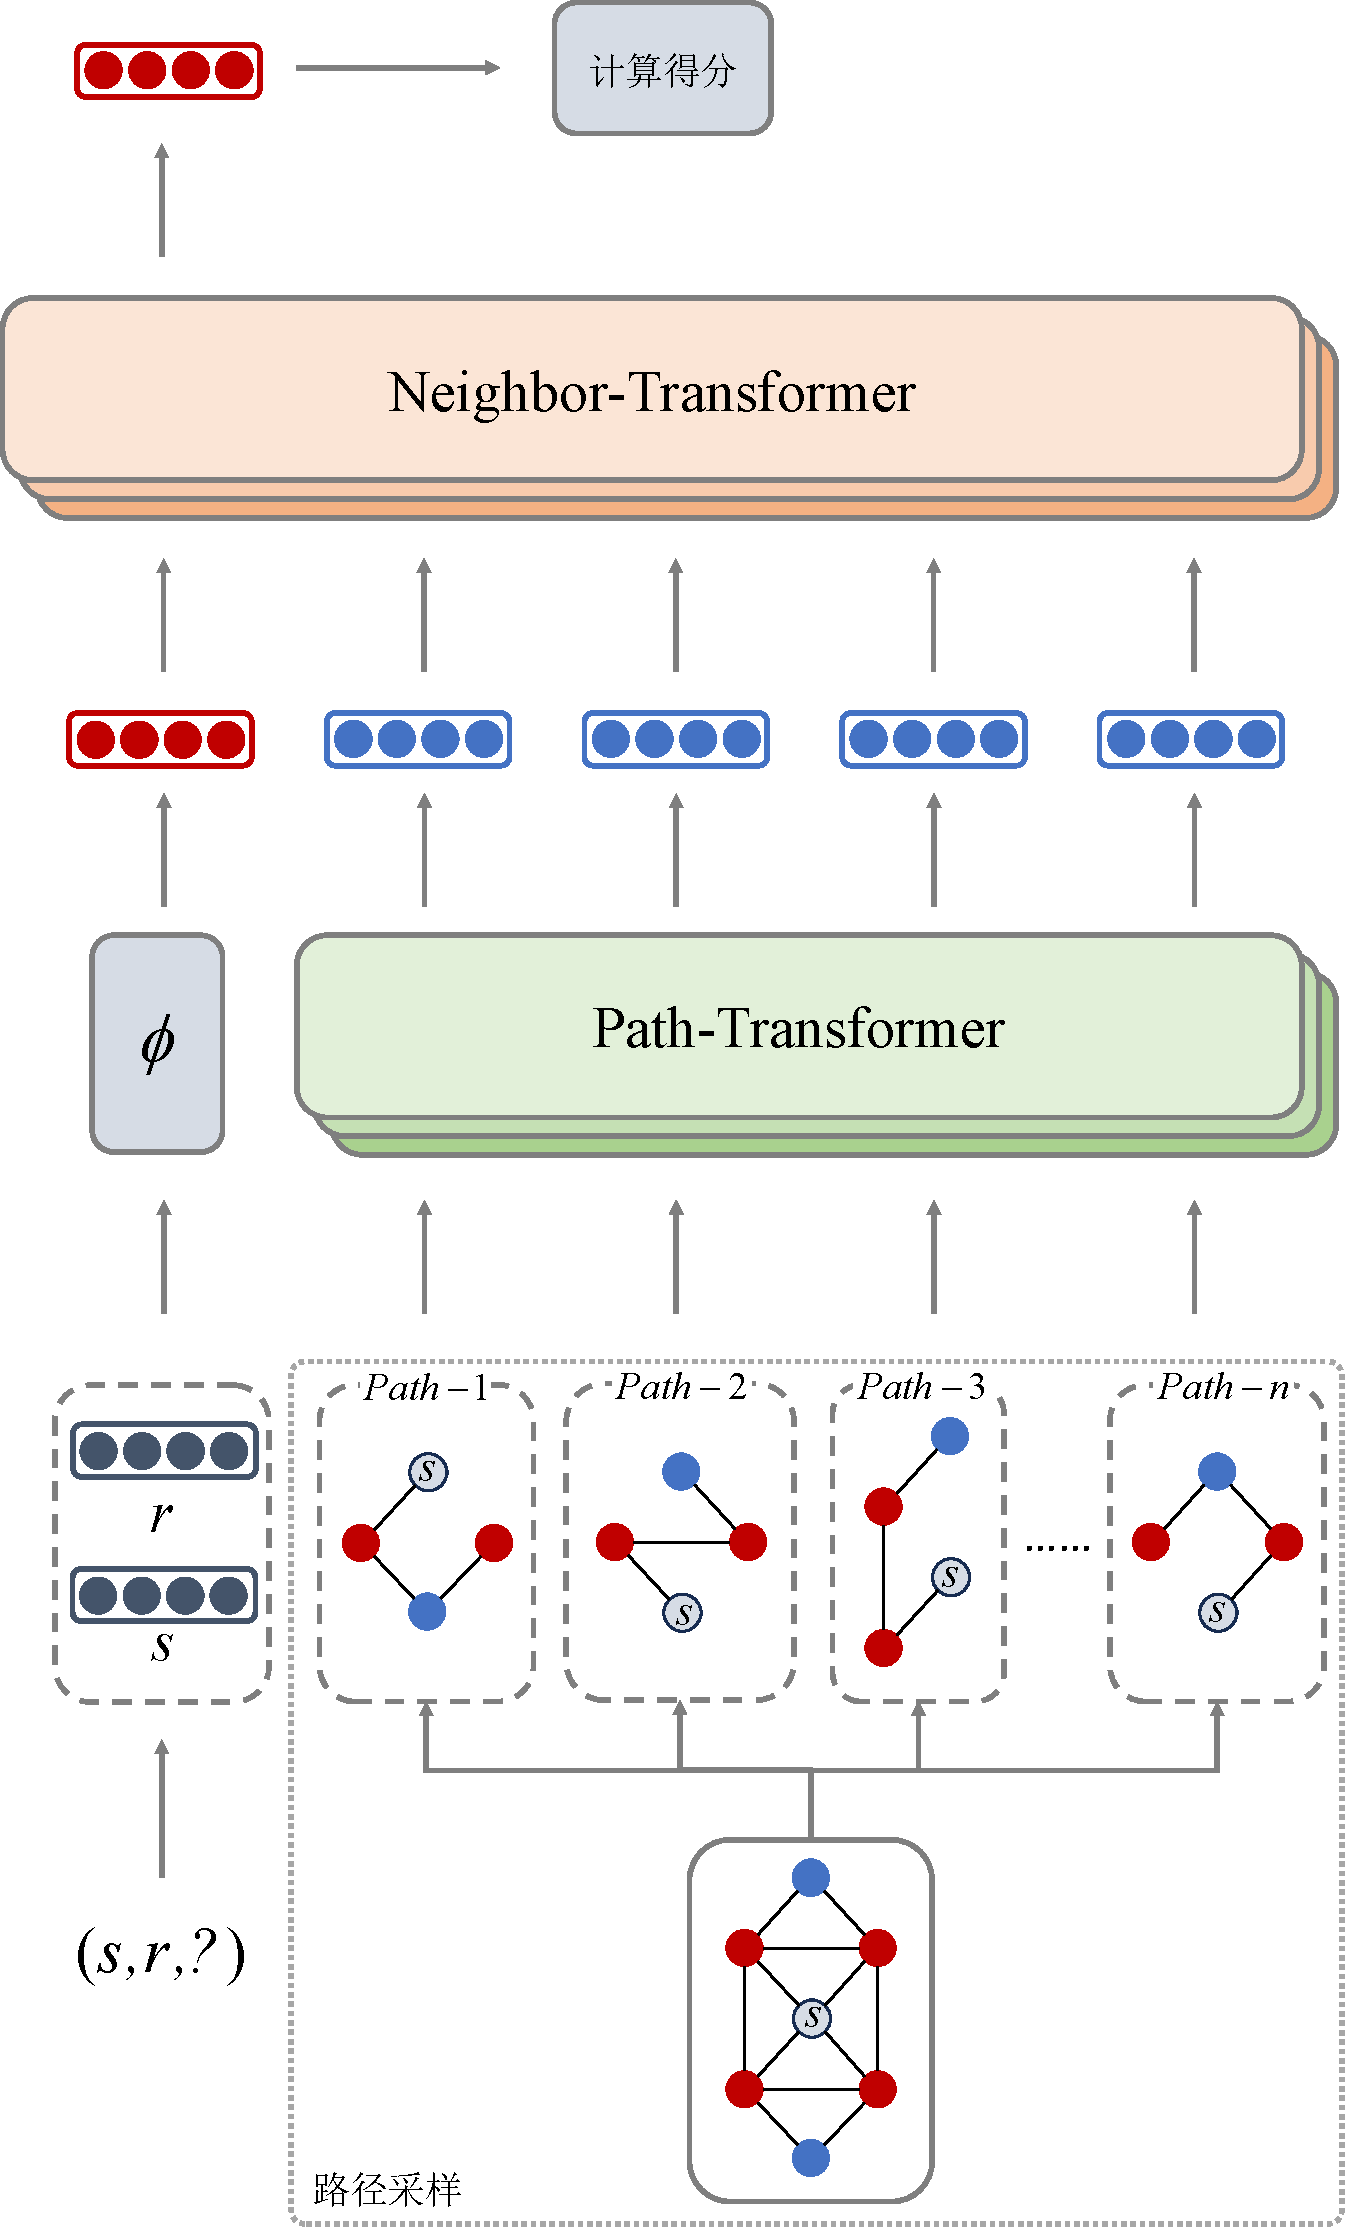
\includegraphics[width=0.65\textwidth]{pic/TKGE-PN_architecture.pdf}}
  \caption{TKGE-PN模型整体架构}
  \label{TKGE-PN_architecture}
\end{figure}

\subsection{基于有偏随机游走的图路径采样算法}

为了通过图路径来学习实体之间的长距离依赖,TKGE-PN模型的第一个任务是获得知识图谱中的图路径信息。由于知识图谱的规模往往十分庞大,因此遍历图谱中所有可能的图路径组合是一件不可能的工作。因此为了让模型能够充分利用图路径信息,提高链路预测的准确性,如何采样到高质量的知识图谱图路径是TKGE-PN首先需要解决的问题。

给定一个待预测的三元组$(s,r,?)$,图路径采样模块的主要任务是获得一条或者若干条以头实体$s$为起点的图路径用于链路预测任务。在TKGE-PN模型中,知识图谱中的图路径被定义为图谱中的实体-关系链,在链中实体和关系交替出现,链的第一个元素和最后一个元素必须为实体。在图谱中,以节点$s$为起点,长度为$T$的图路径$P$表示为:

\begin{equation}
  \begin{aligned}
     &P=<s,r_1,e_1,r_2,e_2,...,r_T,e_T>, \\
     &{\forall}i \in (0,T),e_i\in\mathcal{E},r_i\in\mathcal{R}^{\prime},(e_i,r_{i+1},e_{i+1})\in\mathcal{T}^{\prime}
  \end{aligned}
\end{equation}

以往的基于图路径的知识图谱嵌入方法在给事实三元组打分时利用到的图路径数量往往只有1-2条,例如RSN\upcite{RSN}和Interstellar\upcite{Interstellar}。这些方法采样到的图路径数量相比于知识图谱中可能的图路径数量是十分有限的,因此模型从这些图路径中学习得到的信息往往是片面的,很难全面地挖掘到中心实体对其他实体的长距离依赖,特别是当中心实体的节点度数比较高时,这样的问题会更加严重。此外,并不是所有的路径都对高质量的知识图谱嵌入有意义,低质量的图路径信息可能为引入额外的噪声,反而降低模型的性能。为了解决以上提到这些问题,本文提出了一种基于有偏随机游走的图路径采样算法。

首先,为了解决图路径采样数量不足导致模型学习到的信息不够全面的问题,对于一个待预测的三元组$(s,r,?)$,TKGE-PN的图路径采样模块不再采样固定数量的图路径,而是采样等于头实体$s$的节点度数数量的图路径。一般来说,实体的节点度数越高,以实体作为起点可能采样到的图路径就越多,蕴含的信息就越丰富;而当节点度数较小时,采样一到两条图路径能够充分学习中心实体的长距离依赖。因此随实体节点度数动态变化的图路径采样条数有利于更加全面、有效的捕捉图谱中的长距离依赖信息。

此外,为了避免随机采样的图路径之间出现路径重复而导致信息冗余的情况,对于同一个头实体节点$s$,采样模块确保采样到的不同图路径中的前三个元素组成的事实三元组唯一,即对于不同图路径$P_i=<s,r_1^{i},e_1^{i},...,r_T^{i},e_T^{i}>$和$P_j=<s,r_1^{j},e_1^{j},...,r_T^{j},e_T^{j}>$,有$(s, r_1, e_1)\neq(s, r_2, e_2)$,其中$e_1^{i},e_1^{j}\in \mathcal{N}_s$,$\mathcal{N}_s$为实体 $s$的一阶邻居节点组成的集合。这样的采样方式不仅保证了采样到的图路径之间有足够的区分度,还让采样到的路径覆盖了中心实体的一阶邻域,通过所有采样的图路径,模型就能学习到中心实体的局部邻域信息,实现长短距离依赖的同时学习。

为了确保采样到的图路径能够帮助模型进行链路预测任务,TKGE-PN的图路径采样模块采用有偏随机游走算法来决定图路径中每一跳选中的实体和关系,实现高质量的图路径采样。为了能够更好的捕获长距离的依赖,TKGE-PN希望采样到的路径能够更加的远离起始的头实体,即采样深度更大一些。为了实现这一点,在进行路径采样的过程中,模型提出了深度偏差来控制路径采样的过程。具体来说,假设在图路径采样的过程中,起始节点为$s$,当前选中的实体为$e_i$,上一跳实体为$e_{i-1}$,下一跳的候选实体$e_{i+1}$为$e_i$的一阶邻居,则深度偏差$\mu_{depth}(e_{i+1})$的计算方式为:
\begin{equation}
  \mu_{depth}(e_{i+1})=1-\alpha\cdot\frac{1}{dis(s,e_{i+1})}
\end{equation}
其中$dis(s,e_{i+1})$为实体$s$与实体$e_{i+1}$之间最短路径的距离,$\alpha$为控制采样过程中路径深度的超参数,为了获得深度更大的路径,一般设置为$\alpha>0$,这样候选实体距离起始实体的最短距离越大,则在计算采样概率时的深度偏差越大。图\ref{depth_bias}说明了一个具体的实例。

\begin{figure}[htbp]
  \centerline{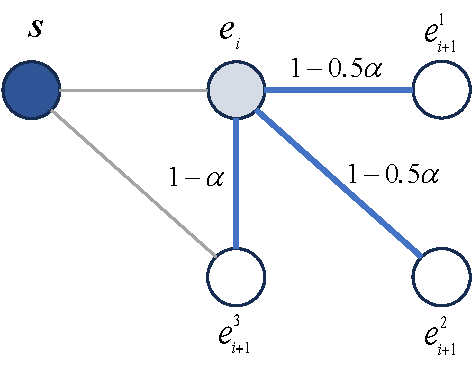
\includegraphics[width=0.5\textwidth]{pic/depth_bias.pdf}}
  \caption{图路径采样过程中的深度偏差}
  \label{depth_bias}
\end{figure}

除了路径深度之外,在图路径采样的过程中,TKGE-PN还将实体的节点度数纳入了考虑。作为知识图谱中一种重要的结构信息,实体的节点度数反映了实体在整个知识图谱中的全局重要性,实体的节点度数越高,说明该实体连接的其他实体和关系越多,蕴含的信息越丰富,应该越重要,为了提高链路预测的准确性,在采样的过程中,节点度数较高的实体采样的权重应该更高。为了实现这一点,模型在路径采样过程中引入了度数偏差。对于候选实体$e_{i+1}$,度数偏差$\mu_{degree}(e_{i+1})$的计算方式如下:
\begin{gather}
  \mu_{degree}(e_{i+1})=\lg(deg_{(e_{i+1})})
\end{gather}
其中$deg_{(e_{i+1})}$为候选实体$e_{i+1}$的度数。此外,我们认为,如果一个实体相邻的实体的节点度数很高,那么该实体的重要性应该也会受到邻居实体的影响随之增加,因为经过该节点可以获取到重要性较高的实体节点的信息,因此在计算度数偏差时TKGE-PN将相邻实体的节点度数也纳入了考虑,有:
\begin{gather}
  \mu_{degree}(e_{i+1})=\frac{1}{2}\lg(deg_{e_{i+1}})+\frac{1}{2\|\mathcal{N}_{e_{i+1}}\|}\sum_{e_k\in\mathcal{N}_{e_{i+1}}}\lg(deg_{e_k})
\end{gather}

最终,我们可以得到在图路径采样的过程中,下一跳候选实体$e_{i+1}$被选中的未正则化的概率计算公式为:
\begin{gather}
  \mu_i = \mu_{depth}(e_{i+1})+\beta\cdot\mu_{degree}(e_{i+1})\\
  p_{sample}(e_{i+1})=\left\{
      \begin{aligned}
          &\mu_i &&\quad (e_i,r_i,e_{i+1})\in \mathcal{T}^{\prime} \\
          &0 &&\quad otherwise
      \end{aligned}
  \right.
\end{gather}
其中$\beta$为控制采样过程中度数偏差的权重。

\subsection{Path-Transformer路径编码模块}

通过基于有偏随机游走的采样算法,TKGE-PN模型获得了若干条图路径用于链路预测任务。但是这些采样到的图路径无法直接使用,还需要Path-Transformer路径编码模块学习其中蕴含的语义信息并转换为对应的向量表示。和处理局部邻域结构不一样的是,图路径天然具有序列数据的形式,而Transformer被认为是建模序列数据的最强大的神经网络,因此原始的Transformer网络就能够很好的挖掘路径中实体与实体、实体与关系之间的长短距离依赖,而无需对网络结构进行额外的改造。

给定一条长度为$T$的图路径$P=<s,r_1,e_1,...,r_T,e_T>$,Path-Transformer路径编码模块的输入主要由以下几个部分组成:图路径嵌入表示$\mathbf{M}_{path} $,以及一个可学习的特殊嵌入Class Token的向量表示$\mathbf{e}_{cls}$用于获取所有输入的统计特性,因此路径编码模块的输入表示为:
\begin{gather}
  \mathbf{M}_{path} = [\boldsymbol{e}_s,\boldsymbol{r}_1,\boldsymbol{e}_1,...,\boldsymbol{r}_T,\boldsymbol{e}_T]\\
  \mathbf{M}_{path}^{\prime} = [\boldsymbol{e}_{cls},\mathbf{M}_{path}]
\end{gather}
其中$\boldsymbol{e}_{cls}\in\mathbb{R}^d$,$\mathbf{M}_{path} \in \mathbb{R}^{(2T+1)\times d}$。$\mathbf{M}_{path}$由图路径中包含的所有的实体及关系对应的嵌入构成,$\boldsymbol{e},\boldsymbol{r} \in \mathbb{R}^d$ 代表分别代表实体和关系嵌入,$d$则为嵌入向量维度的大小。同样的,和NATLP类似,Path-Transformer采用类型嵌入来帮助模型区分实体嵌入,关系嵌入以及特殊嵌入向量$\boldsymbol{e}_{cls}$。此外,由于图路径是序列数据,Path-Transformer采用可学习的位置位置来识别图路径中实体和关系之间的顺序关系,因此Path-Transformer的最终输入表示为:
\begin{equation}
  \mathbf{M}_{input}^{P} = \mathbf{M}_{path}^{\prime}+\mathbf{TE} + \mathbf{PE}
\end{equation}
其中$\mathbf{TE}$ 为类型嵌入,$\mathbf{PE}$为位置嵌入。

在完成输入构造后,Path-Transformer会利用自注意力机制学习图路径中的语义信息。设Path-Transformer模块最后一层的输出为$\mathbf{M}_{output}^{P}\in\mathbb{R}^{(2T+1)\times d}$,TKGE-PN取输出中特殊嵌入向量$\boldsymbol{e}_{cls}$对应位置的嵌入$\boldsymbol{e}_{path}\in\mathbb{R}^d$作为当前图路径的向量表示。

Path-Transformer路径编码模块尝试从知识图谱图路径中挖掘长距离的依赖用于链路预测任务,但是相比于近距离的局部邻域,图路径中蕴含的长距离依赖反应的是实体之间间接的联系,容易在学习的过程中丢失,模型学习起来是更加困难的。针对这样的挑战,受到BERT\upcite{BERT}中掩蔽语言建模(Masked Language Model,MLM)预训练任务的启发,TKGE-PN提出了掩蔽实体关系预测(Masked Entity and Relation Prediction,MERP)任务,以加强Path-Transformer从图路径上下文中挖掘信息的能力。

具体来说,对于输入的每一条图路径$P$,模型将会随机选择遮掩或者替换掉某个关系或者实体进行预测任务。以实体为例,在掩蔽替换阶段,被选中的实体$e_m$ 将会以一定概率被替换成特殊的掩蔽占位嵌入$e_{mask}$、其他的随机实体或者维持不变,模型使用超参数来调节以上三种情况的概率。而在预测阶段,模型取Path-Transformer输出嵌入矩阵$\mathbf{M}_{output}^{P}$中被选中的实体对应的嵌入$\boldsymbol{e}_{m}^\prime$来尝试辨认出被遮掩的正确实体$e_m$。具体来说,对于一个候选的实体$e_t$,模型将$\boldsymbol{e}_{m}^\prime$通过一个双层全连接层并计算$\boldsymbol{e}_{m}^\prime$与$\boldsymbol{e}_{t}$之间的余弦相似度来获得候选实体$e_t$的正确概率$p_m$:
\begin{equation}
  p_m(e_t)=\sigma((f(\boldsymbol{e}_m^\prime\mathbf{W}^{\prime})\mathbf{W}^{\prime\prime})\boldsymbol{e}_t)
\end{equation}
其中$f (\cdot)$和$\sigma(\cdot)$分别代表ReLU和sigmoid激活函数,$\mathbf{W}^{\prime}$和$\mathbf{W}^{\prime\prime}$分别为两个全连接层的参数。当被选中的元素为关系时,处理方法类似。最后TKGE-PN通过交叉熵损失函数,计算得到掩蔽实体关系预测任务的分类损失为:
\begin{equation}
  L_{P} = -\frac{1}{N}\sum\limits_{i}t_m^ilog(p_m^i)+(1-t_m^i)log(1-p_m^i)
\end{equation}
其中$t_m^i$为MERP任务中的分类标签,$p_m^i$为对应候选实体的正确概率。

掩蔽实体关系预测任务加强了Path-Transformer挖掘图路径中语义信息的能力。在原本的训练过程中,由于近距离的依赖学习难度较低,模型可能会倾向于挖掘近距离的实体中蕴含的信息,而忽略了远距离的部分。而通过随机地对图路径中的元素进行掩蔽,模型无法再单纯地依赖某个特定的图路径元素;通过对掩蔽的元素进行预测,模型也确保了信息不会丢失。基于掩蔽实体关系预测任务,模型实现了对图路径中长短距离依赖信息的平衡。

\subsection{Neighbor-Transformer局部邻域编码模块}

给定一个待遇测的三元组$(s,r,?)$,通过基于有偏随机游走的图路径采样算法,模型已经获得了以头实体$s$为起点的多条图路径,数量等于头实体$s$的节点度数。通过对采样的规则进行限制,这些图路径覆盖了头实体$s$的一阶局部邻域。因此,Neighbor-Transformer局部邻域编码模块通过基于Path-Transformer学习到的所有的图路径表示,便能够同时结合知识图谱的局部邻域结构信息和图路径结构信息,在避免过平滑问题的同时实现对于长短距离依赖的同时学习,提高知识图谱补全任务的性能。

Neighbor-Transformer局部邻域编码模块的输入主要包含以下几个部分:图路径嵌入矩阵$\mathbf{M}_{paths}$,查询嵌入$\boldsymbol{e}_{query}$以及一个可学习的特殊嵌入$\boldsymbol{e}_{gcls}$。$\mathbf{M}_{paths}\in\mathbb{R}^{N_p\times d}$由所有采样到的以头实体$s$为起点的图路径的嵌入表示组成,其中$N_p$为采样到的图路径的数量,有:
\begin{equation}
  \mathbf{M}_{paths}=\left[ \boldsymbol{e}_{P_1},\boldsymbol{e}_{P_2},...,\boldsymbol{e}_{P_{N_p}}\right]
\end{equation}
其中$\boldsymbol{e}_{P_i} \in \mathbb{R}^d$为第$i$条图路径的向量表示。为了能够发挥Transformer模型的表达能力,避免模型的性能被基于卷积神经网络的解码器限制,TKGE-PN抛弃了NALTP中采用的编码器-解码器架构,而是利用Transformer网络尝试直接拟合待遇测尾实体$o$的嵌入。查询向量$\boldsymbol{e}_{query}$的主要作用是向Transformer传递待遇测三元组的信息,让模型能够基于当前输入调整注意力分数的计算,提高模型链路预测的性能。$\boldsymbol{e}_{query}$由待预测三元组中头实体$s$和关系$r$对应的嵌入向量$\boldsymbol{s}$和$\boldsymbol{r}$计算得到,有:
\begin{equation}
  \boldsymbol{e}_{query}=\varPhi(\boldsymbol{s},\boldsymbol{r})
\end{equation}
其中$\boldsymbol{s},\boldsymbol{r}\in\mathbb{R}^d$,$\varPhi(\cdot)$为对应的运算函数,可以根据不同的场景选用不同的形式,例如向量相加,向量相乘,或者利用神经网络完成查询向量的构造。本文中采用的是NATLP中基于特定关系的消息构造方式,有:
\begin{equation}
  \varPhi \left(s,r\right) = f\left(vec\left(f\left(\phi_{chk}\left(\boldsymbol{s},\boldsymbol{r}\right) \circledast \omega_{r} \right)\right)\mathbf{W}_{r}\right)
\end{equation}

特殊嵌入向量$\mathbf{e}_{gcls}$用于获取所有输入的统计特性,并且对应位置的输出将会被用于链路预测任务最后的概率计算。和NALTP类似,三种不同的类型嵌入被用来区分图路径嵌入矩阵$\mathbf{M}_{paths}$,查询嵌入$\boldsymbol{e}_{query}$以及$\boldsymbol{e}_{gcls}$。由于不同的图路径信息之间没有明显的相对位置关系,因此Neighbor-Transformer局部邻域编码模块中没有使用位置嵌入。最终,Neighbor-Transformer模块的输入表示为:
\begin{gather}
  \mathbf{M}_{neighbor}^{\prime}=[\boldsymbol{e}_{gcls},\boldsymbol{e}_{query},\mathbf{M}_{paths}]\\
  \mathbf{M}_{input}^{N}=\mathbf{M}_{neighbor}^{\prime}+\mathbf{TE}
\end{gather}

和NATLP类似,考虑到图路径上的实体度数之和能够一定程度上反应图路径信息的重要性,在计算注意力分数时,Neighbor-Transformer将图路径的整体节点度数也纳入了考虑。具体的,Neighbor-Transformer在计算注意力得分时额外添加一个图路径节点度数的辅助项:
\begin{gather}
  a_{ij}=\frac{(\boldsymbol{e}_{P_i}W_Q)(\boldsymbol{e}_{P_j}W_K)^T}{\sqrt{d}}+1-\frac{1}{\lg (deg_{P_i})\cdot \lg (deg_{P_j})}\\
  deg_{P_i}=\sum_{n = 1}^{T}  deg_{e_n}
\end{gather}

最后,TKGE-PN取最后一层输出中对应特殊嵌入向量$\boldsymbol{e}_{gcls}$对应位置的输出向量$\boldsymbol{T}_{GCLS}$来进行链路预测任务。对于任意一个候选实体$e_t$,模型将$\boldsymbol{T}_{GCLS}$与$e_t$的嵌入$\boldsymbol{e}_{t}$进行点积后并经过sigmoid激活函数后得到三元组$(s,r,e_t)$的得分$p$。获得所有候选实体的得分后,计算得到链路预测任务的交叉熵损失为:
\begin{equation}
  L_{LP} = -\frac{1}{N}\sum\limits_{i}t_ilog(p_i)+(1-t_i)log(1-p_i)
\end{equation}
最终,通过将链路预测任务的损失和掩蔽实体关系预测任务的损失相加,我们可以得到用于模型训练的最终损失函数:
\begin{gather}
  L_{MERP} = -\frac{1}{N_p}\sum\limits_{i}L_{p_{i}}\\
  L=L_{LP}+L_{MERP}
\end{gather}
其中$L_{p_{i}}$是第$i$条图路径上掩蔽实体预测任务的损失。

此外,为了避免出现模型训练和模型预测时的数据分布的不一致,在训练过程中模型将从头实体的邻域内移除真实的尾实体,避免训练期间模型总是可以从头实体的邻域内感知到真实的尾实体,而这种情况和预测时的实际情况不符。


\section{本章小结}

本章对TKGE-PN模型的整体架构和实现细节进行了详细介绍。首先对基于图神经网络的方法以及前文提出的NATLP模型依然存在的问题进行了介绍;随后给出了模型中涉及到的数学符号的详细定义;之后介绍了模型的整体架构组成;最后,对TKGE-PN中的关键设计细节进行了具体的说明,包括(1)基于有偏随机游走的图路径采样算法,将图路径的路径深度以及实体的节点度数纳入了考虑,用于采样高质量的图路径(2)Path-Transformer路径编码模块,通过掩蔽实体关系预测任务加强模型学习图路径中语义信息的能力,实现了长短距离依赖信息的平衡(3)Neighbor-Transformer局部邻域编码模块,结合待遇测的事实三元组,综合图路径结构信息和局部邻域结构信息完成链路预测任务。


\chapter{TKGE-PN模型实验与验证}
为了验证本文提出的TKGE-PN算法能够通过结合图路径和局部邻域信息实现对知识图谱中的长短距离依赖的综合学习,提高链路预测任务的性能表现,本文在两个基准数据集上对TKGE-PN进行了实验验证。TKGE-PN模型实验时采用的数据集、实验环境和评估策略和NATLP模型实验时完全一致,因此本章不再另行介绍。本章首先说明了用来对比的基线算法以及模型在两个数据集上的超参数设置,随后介绍了模型的整体实验结果并进行了深入的探究,最后通过消融实验对模型的关键设计进行了分析和讨论。

\section{实验方案设计}

\subsection{对比算法}

为了验证本文提出的TKGE-PN模型在链路预测任务上的有效性,在实验部分,本文将其与一些最具代表性的以及最先进的知识图谱嵌入模型进行了比较,主要包含以下几类:

(1)传统的知识图谱嵌入模型,时间和空间复杂度较低,包括基于翻译的模型TransE\upcite{TransE},RotatE\upcite{RotatE},基于张量分解的模型DistMult\upcite{DistMult},ComplEx\upcite{ComplEx},以及基于卷积神经网络的模型ConvE\upcite{ConvE}和ConvR\upcite{ConvR}。

(2)基于图神经网络的嵌入模型,主要学习图谱局部邻域结构进行知识图谱嵌入,包括R-GCN\upcite{R-GCN},CompGCN\upcite{CompGCN},KBGAT\upcite{KBGAT},HKGN\upcite{HKGN},SE-GNN\upcite{SE-GNN}以及MRGAT\upcite{MRGAT}。

(3)基于图路径的嵌入模型,利用知识图谱的图路径结构进行嵌入工作,包括RSN\upcite{RSN}和Interstellar\upcite{Interstellar}。 

(4)基于Transformer的嵌入模型,主要利用Transformer的表达能力进行链路预测,包括KG-BERT\upcite{KG-BERT},HittER\upcite{HittER},StAR\upcite{StAR}和Relphormer\upcite{Relphormer},以及本文先前提出的NALTP模型。

\subsection{模型超参数设置}

实验采用的超参数是通过网格搜索在验证集上进行评估后得出的。实验中,Path-Transformer图路径编码模块以及Neighbor-Transformer局部邻域编码模块分别由3层和4层Transformer编码层组成,多头注意力机制的头数为8,采用的实体和关系嵌入维度为320。在路径采样算法的设置上,两个数据集上路径采样的深度偏差权重$\alpha = 0.7$,度数偏差权重$\beta=0.1$,WN18RR数据集上采样路径的最大长度$T=4$,FB15k-237数据集上$T=3$。在掩蔽实体关系预测任务中,每个实体和关系有30\%的概率被特殊的掩蔽占位嵌入$e_{mask}$替换,20\%被其余随机实体和关系替换,50\%的概率维持不变。考虑到数据集中存在极小一部分节点度数极高的实体以及FB15k-237和WN18RR数据集在节点平均度数上的差异,实验对每个实体采样得到的图路径的最大数量进行了限制,在FB15k-237和WN18RR数据集上分别为50和12,这样的设置能够保证采样的图路径可以完全覆盖数据集中80\%以上实体的一阶邻域。

实验中采用了Adamax\upcite{Adamax}优化器结合动态学习率调整策略进行模型的训练。在总迭代次数的前10\%内,模型的学习率将从0线性提升到最高,并在剩余迭代次数内线性下降到0。在训练过程中,除了嵌入层以外的神经网络层的随机失活概率为0.65,嵌入层的随机失活概率为0.2。模型训练时在FB15K-237数据集上的总迭代次数为300,训练批次的大小为512,最大学习率为0.0011;而对于WN18RR数据集,总迭代次数为500,批处理大小为512,最大学习率为0.002。为了防止模型出现过度自信的现象,训练过程中以0.1的比率进行了标签平滑。模型使用的具体超参数参见表\ref{TKGE-PN_hyperparameter}。

\begin{table}[htbp]
    \renewcommand\arraystretch{1.5}
    \caption{TKGE-PN模型超参数设置}
    \centering
    \begin{tabular}{*{3}{c}}
      \toprule
      超参数 & FB15k-237 & WN18RR\\
      \midrule
      实体和关系嵌入大小  & 320 & 320 \\
      Path-Transformer网络层数& 3 & 3\\
      Neighbor-Transformer网络层数& 4 & 4\\
      嵌入层Dropout概率 & 0.2 & 0.2\\
      Transformer中的Dropout概率 & 0.65 & 0.65\\
      采样路径的最大长度&3 &4\\
      深度偏差权重& 0.7 & 0.7\\
      度数偏差权重& 0.1 & 0.1\\
      路径采样最大数量 &50&12\\
      训练批次大小 & 512 & 512\\
      总迭代次数& 300 & 500 \\
      最大学习率 & 0.001 & 0.02\\
      标签平滑比例 & 0.1 & 0.1\\
      \bottomrule
    \end{tabular}
    \label{TKGE-PN_hyperparameter}
  \end{table}

\section{实验结果与分析}

\subsection{整体实验结果分析}

不同模型在WN18RR数据集和FB15k-237数据集上的链路预测实验结果如表所示。和NATLP类似,TransE、RotatE、DistMult、ComplEx和ConvE在两个数据集上的实验结果直接选取文献\cite{49}中经过大量调参的最优结果。由于存在评估策略不当以及测试集数据泄露的问题,KBGAT的实验结果选取文献\cite{50}中经过修正后的结果。

\begin{table}[htbp]
    \begin{center}
        \caption{TKGE-PN实验结果}
        \renewcommand\arraystretch{1.5}
        \setlength{\tabcolsep}{5pt}
        \begin{tabular}{*{11}{c}}
            \toprule
            \multirow[vpos]{2}{*}[-0.8ex]{模型} & \multicolumn{5}{c}{WN18RR} & \multicolumn{5}{c}{FB15k-237}\\
            \cmidrule(lr){2-6}\cmidrule(lr){7-11}
            &MRR & MR & Hits@1 &Hits@3 & Hits@10&MRR & MR & Hits@1 &Hits@3 & Hits@10\\
            \midrule
            TransE&0.228&-&0.053&0.368&0.520&0.313&-&0.221&0.347&0.497\\
            RotatE&0.478&-&0.439&0.494&0.553&0.333&	-&0.240&0.368&0.522\\
            DistMult&0.452&-&0.413&0.466	&0.530	&0.343	&-	&0.250	&0.378	&0.531\\
            ComplEx&0.475&-&0.438	&0.490	&0.547	&0.348	&-	&0.253	&0.384	&0.536\\
            ConvE&0.442&-&0.411&0.451	&0.504&	0.339	&-&	0.248&	0.369	&0.521\\
            ConvR&0.475&-&0.443&	0.489&	0.537&	0.350&	-&	0.261&	0.385&	0.528\\
            \cmidrule{1-11}
            R-GCN & -&-&-&-&-&0.248&-&0.153&0.258&0.414\\
            CompGCN&0.479&3533&0.443	&0.494	&   0.546&	0.355	&197	&0.264	&0.390&	0.535\\
            KBGAT&0.412&1921&-&	-&	0.554	&0.157	&270	&-&	-&	0.331\\
            SE-GNN&0.484&3211&0.446&	0.509&	0.572	&0.365& 157	&0.271	&0.399	&0.549\\
            MRGAT&0.481&-&0.443&0.501&0.568&0.358	&-&0.266&0.386&0.542\\
            HKGN&0.487&2468&0.448&0.505&0.561&0.365&194&0.271&0.397&0.544\\
            \cmidrule{1-11}
            RSN&0.400&-&0.380	&-	&0.448&	0.280	&-	&0.202	&-	&0.453\\
            Interstellar&0.480&-&0.438	&-	&0.546	&0.320	&-	&0.233	&-	&0.508\\
            \cmidrule{1-11}
            KG-BERT&0.216&\underline{97}&0.041&	0.302	&0.524	&-	&\underline{153}	&-&	-&	0.420\\
            HittER&0.503&-&0.462&	0.516&	0.584	&0.373	&-	&0.279	&0.409	&0.558\\
            StAR&0.40&\textbf{51}&0.243	&0.491	&0.709	&0.296	&\textbf{117}&	0.205	&0.322	&0.482\\
            Relphormer&0.495&-&0.448&	-	&\textbf{0.591}&	0.371		&-&\textbf{0.314}	&-	&0.481\\
            \cmidrule{1-11}
            NATLP&\underline{0.505}&2687&\underline{0.465}&\underline{0.519}&0.576&\underline{0.374}&181&0.281&\underline{0.411}&\underline{0.560}\\
            \textbf{TKGE-PN}&\textbf{0.510}&2540&\textbf{0.467}	&\textbf{0.522}	&\underline{0.590}	&\textbf{0.379}	&160	&\underline{0.288}	&\textbf{0.414}	&\textbf{0.562}\\
            \bottomrule
        \end{tabular}
        \label{TKGE-PN_result_tab}
    \end{center}
  \end{table}

  表中加粗项为每项指标的最高值,下划线项为每项指标的次高值。从表\ref{TKGE-PN_result_tab}中可以观察到,(1)在两个基准数据集中的大多数评价指标上,TKGE-PN模型优于其他所有的基准模型,这证明了本文提出的方法的有效性。TKGN-PN和NATLP等基于Transformer的嵌入方法相比于基于图卷积神经网络的嵌入方法如MRGAT取得了较大的性能提升,这证明了Transformer结构在知识图谱嵌入领域的巨大潜力。(2)而同样是基于Transformer的知识图谱嵌入方法,NALTP利用Transformer来学习中心实体的一阶邻域信息,没有利用路径信息而缺乏捕捉图谱中长距离依赖的能力。TKGE-PN相对于NALTP的性能提升表明了图路径结构对于知识图谱嵌入的帮助以及TKGE-PN从图路径结构中挖掘长距离依赖的能力。

  为了进一步研究图路径采样策略对于TKGE-PN链路预测性能的影响,本文探究了在不同图路径采样长度下TKGE-PN在两个数据集上的性能表现,实验结果如表\ref{length_tab}所示。

\begin{table}[htbp]
    \begin{center}
        \caption{验证集上不同路径采样长度下的链路预测结果}
        %\setlength{\tabcolsep}{12pt}
        \renewcommand{\arraystretch}{1.5}
        \begin{tabular}{*{5}{c}}
            \toprule
            采样路径的最大长度& \multicolumn{2}{c}{WN18RR} & \multicolumn{2}{c}{FB15k-237}\\
            \cmidrule(lr){2-3}\cmidrule(lr){4-5}
            $T$&MRR&Hits@10&MRR&Hits@10\\
            \midrule
            1	&0.498&0.571&0.373&0.559\\
            2	&0.503&0.580&0.376&0.560\\
            3	&0.506&0.584&\textbf{0.380}&\textbf{0.563}\\
            4	&\textbf{0.509}&\textbf{0.588}&0.377&0.561\\
            5	&0.507&0.585&0.375&0.557\\
            6	&0.503&0.578&0.372&0.559\\
            7	&0.501&0.576&0.370&0.555\\
            \bottomrule
        \end{tabular}
        \label{length_tab}
    \end{center}
\end{table}
  
可以发现,随着采样长度的增加,模型在两个数据集上的性能总体呈现一个先上升后降低的趋势。一方面,路径长度的增加能够帮助模型学习到长距离的依赖,因此在初期能够有效提升模型嵌入效果;而另一方面,并不是所有的图路径信息都是有意义的,采样长度过高时采样到的路径随机性会增大,距离过长时两个实体之间的依赖也会减弱,引入的噪声信息随之增加,反而对模型造成了干扰,导致性能下降。此外,根据实验结果可以发现,在不同数据集上模型最优的采样长度也不同,相比较之下,WN18RR数据集上的最优长度更大。本文认为这样的差异是由于不同数据集之间的稀疏性差距导致的,WN18RR数据集相对更加稀疏,使得采样的随机性降低,引入的噪声数据减少,因此最优的采样长度相比于FB15k-237数据集更大。

此外,论文还探究了不同路径深度偏差$\alpha$下TKGE-PN模型的性能表现。深度偏差$\alpha$较小时路径采样偏向于围绕中心实体进行,深度偏差$\alpha$较大时则更注重于捕捉远距离的依赖。根据实验结果,论文发现当深度偏差$\alpha\in\left[0.6,0.8\right] $时模型的性能表现最好。本文认为当深度偏差控制在这个区间内时,模型能够比较好的兼顾长短距离的信息。

\subsection{模型关键设计分析}

为了验证TKGE-PN模型中局部邻域、图路径信息以及掩蔽实体关系预测任务对于知识图谱嵌入的作用,论文在两个数据集上分别以四种设置进行了消融实验,分别是未消融任何部分的TKGE-PNM模型、去除了局部邻域编码模块、去除掩蔽实体关系预测任务以及同时去除图路径编码模块和掩蔽实体关系预测任务,实验结果如表\ref{ablation_tab}所示。

\begin{table}[htbp]
    \begin{center}
        \caption{TKEG-PN消融实验结果}
        \setlength{\tabcolsep}{10pt}
        \renewcommand{\arraystretch}{1.5}
        \begin{tabular}{*{7}{c}}
            \toprule
            数据集 & 模型 & MRR&MR&Hits@1&Hits@3&	Hits@10\\
            \midrule
            \multirow{4}{*}{WN18RR}&TKGE-PN&0.509&2610&0.467&0.525&0.588\\
            &Path+MERP&0.487&2752&0.445&0.504&0.567\\
            &Neighbor&0.497&2806&0.459&0.512&0.570\\
            &Neigbor+Path&0.502&2636&0.461&0.521&0.579\\
            \cmidrule{1-7}
            \multirow{4}{*}{FB15k-237}&TKGE-PN&0.380&156&0.289&0.415&0.563\\
            &Path+MERP&0.367&144&0.278&0.406&0.555\\
            &Neighbor&0.373&175&0.279&0.410&0.559\\
            &Neigbor+Path&0.376&169&0.282&0.413&0.562\\
            \bottomrule
        \end{tabular}
        \label{ablation_tab}
    \end{center}
\end{table}

具体来说,去除局部邻域编码模块是通过限制路径采样数量为1来实现,而去除图路径编码模块则是通过限制路径采样长度为1实现,此时路径信息内只包含中心实体的一阶邻居,即一阶局部邻域信息。可以看到,无论是去除局部邻域编码模块,还是去除图路径编码模块,模型的效果都会出现明显的降低。实验证明了知识图谱中的这两种结构信息都能够帮助进行链路预测,仅依赖路径信息,模型无法从局部邻域内的丰富的实体和关系中学习到中心实体的综合性质;仅依赖局部邻域,则无法挖掘到中心实体和其他实体之间的远距离依赖。相对来说,去除局部邻域编码模块带来的性能下降更加的严重,这证明了局部邻域信息的重要性,也符合一般的直觉:距离中心实体更近的实体和关系更能反映中心实体的性质,蕴含的信息也更加容易学习。此外,论文发现在脱离掩蔽实体关系预测任务的情况下添加图路径信息而并不能带来明显的性能提升,这说明了图路径上长距离信息学习的困难性以及掩蔽实体关系预测对提升模型长距离信息学习能力的作用。总体来看,TKGE-PN模型任一部分的缺失都会导致模型的最终结果受到负面影响。

为了进一步验证图路径信息在挖掘知识图谱中长距离依赖的作用,以及长距离依赖信息对于链路预测任务的帮助,本文将WN18RR验证集中的事实三元组按照头实体和尾实体之间的最短距离进行了划分,并在划分后的验证集上评估了消融了路径编码模块的TKGE-PN模型以及原始TKGE-PN模型的链路预测任务性能,实验结果如图\ref{tkge_experiment}所示。

\begin{figure}[htb]
    \centerline{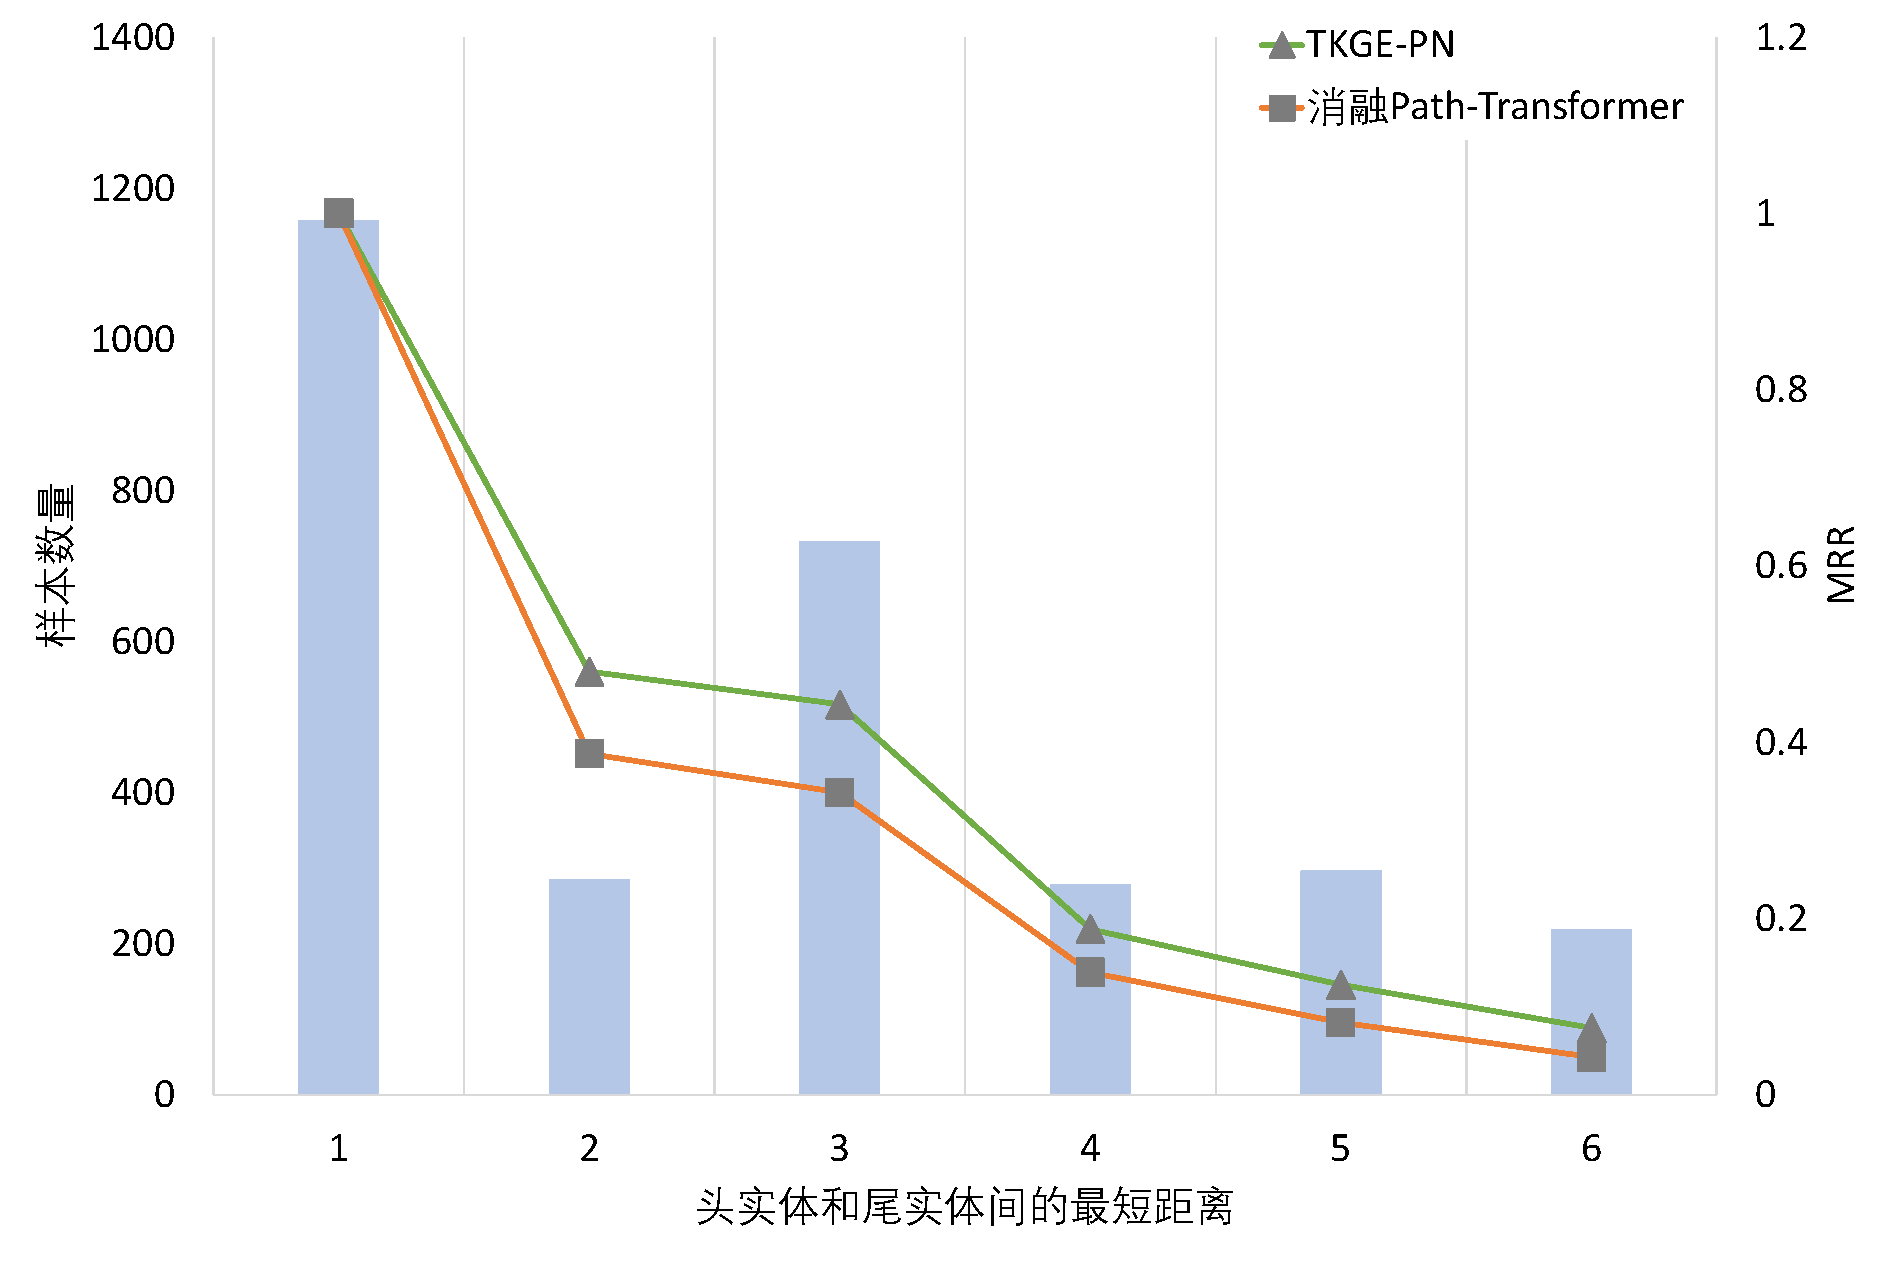
\includegraphics[width=1\textwidth]{pic/TKGE-PN_experiment.pdf}}
    \caption{WN18RR分组实验结果}
    \label{tkge_experiment}
  \end{figure}

从图\ref{tkge_experiment}中实验结果可以发现,随着头实体和尾实体之间最短距离的增加,模型的MRR指标出现了明显的下降,说明推断图谱之间的长距离依赖是非常困难的。 此外,可以注意到的是,相比于消融了图路径编码模块的模型,学习了图路径的TKGE-PN模型在长距离的样本上性能表现更好,特别是在头尾实体间最短距离为2-4的样本上,证明了图路径信息能够有效捕捉实体间的长距离依赖,提高链路预测任务的性能表现。

\section{本章小结}

本章对于结合图路径和局部邻域的Transformer模型TKGE-PN的实验部分进行了介绍,首先介绍了用来对比的基线模型以及模型在两个数据集上的超参数设置。之后论文对TKGE-PN模型的整体实验结果进行了介绍,证明了TKGE-PN模型性能表现优于绝大部分现有的模型。论文随后通过实验进一步探究了路径长度以及路径采样策略对于TKGE-PN性能的影响;最后论文通过实验对TKGE-PN模型中的关键设计进行了具体的探究和分析,包括图路径编码模块、局部邻域编码模块以及掩蔽实体关系预测任务,并设计了实验证明了图路径在长距离依赖信息学习中的重要作用。

% 总结
% !TeX root = ../Template.tex
% 总结
\summary
% 自从2017年被提出,Transformer已经在计算机视觉、自然语言处理等多个领域大放异彩,展现出了巨大的潜力,收到了许多的关注,因此也有不少工作尝试将Transformer网络引入到知识图谱补全领域中。
本课题针对传统知识图谱嵌入方法和基于图神经网络的方法的缺点,研究如何利用Transformer模型来学习知识图谱中的语义和结构信息,提升知识图谱补全任务的性能,提出了两种新型的基于Transformer的知识图谱补全方法:基于邻域感知的Transformer模型NATLP,并在NATLP模型的基础上进一步提出了结合图路径和局部邻域的Transformer模型TKGE-PN。

针对基于图神经网络的知识图谱嵌入方法表达能力不足的问题,NATLP研究利用Transformer网络来完成知识图谱补全。针对以往模型对关系和实体间的交互建模不足的问题,NATLP在模型输入信息构造阶段,基于关系生成特定的网络参数,实现关系特定的邻居信息构造,显示建模了不同关系对于实体传递消息的影响;针对Transformer无法直接感知图结构的问题,NALTP对Transformer的自注意力机制进行了改造,提出了一种融合图结构的自注意力机制,使得模型能够学习到输入消息之间的互相依赖;

NATLP模型解决了基于图神经网络的模型存在的部分问题,但依然无法有效学习图谱中的长距离依赖。针对基于图神经网络的方法和NATLP方法中的以上缺陷,本文在NATLP的基础上进一步提出了结合图路径和局部邻域的Transformer模型TKGE-PN。TKGE-PN通过对知识图谱中的局部邻域和图路径两种结构信息的融合,完成了在利用丰富的邻域信息的同时对于图谱中长距离信息的挖掘,提高了知识图谱补全任务的性能。TKGE-PN首先通过基于有偏随机游走的采样算法对图路径进行采样,随后通过基于Transformer的图路径编码模块学习其中的长距离依赖,并通过掩蔽实体关系任务实现长短距离信息的平衡;最后通过局部邻域编码模块实现了图路径和局部邻域结构信息的综合应用。

实验结果表明,在两个标准数据集WN18RR和FB15k-237上,NATLP和TKGE-PN的链路预测任务的性能表现超越绝大多数现有的嵌入模型,证明了本文提出的两个模型以及其中的关键设计的有效性。

% 未来,我们计划进一步探索对于知识图谱中结构信息的利用,包括更有效率的利用方式和更加丰富的结构信息种类,同时尝试将TKGE-PN应用到除链路预测之外的其他知识图谱表示学习任务中。

本文涉及的研究内容还有许多可以拓展的地方。首先,知识图谱的图结构除了图路径和局部邻域之外还有其他的表现形式,我们计划进一步探索对于知识图谱中结构信息的利用,例如在规模更大的子图范围上来应用Transformer网络,进一步挖掘模型的潜力。

其次,除了结构信息之外,知识图谱中也蕴含着丰富的文本信息,例如实体的文字描述。而Transformer网络被广泛应用于预训练语言模型中,在挖掘文本语义信息方面存在天然优势。未来我们计划研究将模型与预训练语言模型进行结合,同时利用文本信息和图结构信息来完成知识图谱补全任务。

最后,Transformer网络的复杂度较高,训练和预测时的开销较大,在处理大规模知识图谱时可能会遇到资源上的瓶颈。因此如何优化基于Transformer的结构带来的大量资源开销也是一个值得研究的方向。



% 参考文献
% 手册中参考文献标准似乎并没有严格按照国标GBT7714-2015执行
\Bib{bst/GBT7714-BUAA}{ref}

% 攻读学位期间成果
% !TeX root = ../Template.tex
% [攻读学位期间取得的成果]
\achievement
\noindent
[1] Liu X, \textbf{Zhu T}, Tan H, et al. Heterogeneous graph neural network with hypernetworks
for knowledge graph embedding [C]//The Semantic Web–ISWC 2022: 21st International
Semantic Web Conference, Virtual Event, October 23–27, 2022, Proceedings. Berlin,
Heidelberg: Springer-Verlag, 2022: 284–302

\noindent
[2] 郭子溢,\textbf{朱桐},林广艳,等. 球面坐标下基于语义分层的知识图谱补全方法 [J]. 应用科学学报, 2024, 42 (01): 119-133.



% 致谢
% !TeX root = ../Template.tex
% [致谢]
\acknowledgments

研究生三年生涯转瞬即逝,我的学生生涯也马上要走到了尽头。回首过去的三年,我初次叩开了科研的大门,虽然未能深入探索,但也收获良多,受益匪浅。

在三年的研究生生活中,我首先要感谢的是谭火彬老师和林广艳老师对我的学术和生活上给予的指导和帮助。两位老师不仅会在学术上为我提供建议,指明方向,对我的论文提出了许多宝贵的修改意见,生活中,还时刻关心着我们的身体健康和心理状况,在我的职业规划上也提供了大力的支持。实验室的良好氛围也为我提供了非常好的学习和研究的环境。能够接受两位老师的指导是我的幸运。还要感谢我的父母,他们的默默付出是我最坚强的后盾,父母的理解和爱护是我低谷时最重要的慰藉和支持。

此外,我还要感谢实验室的各位同门。感谢刘希阳学长在我初入实验室时提供的指导,帮助我迈出了学术研究的第一步,在我论文工作遇到困难时也对我提出了非常宝贵的意见和建议。还要感谢柳啸峰、郭子溢、朱伯同三位学长在我的学术研究中为我答疑解惑,学长们丰富的经验帮助我少走了不少弯路。感谢任博林和蒋沛宇两位学弟,论文实验的顺利完成离不开他们对于实验室服务器的维护。

最后,我要感谢我的小伙伴们,三年的时间我们一起度过了一段难忘的时光。




\vspace{5cm}

\end{document}
